%%%%%%%%%%%%%%%%%%%%%%%%%%%%%%%%%%%%%%%%%%%%%%%%%%%%%%%%%%%%%%%%%%%%%%%%%%%%%%%%%%%%%%%%%%%%%%%%%%%
%%%%%%%%%%%%%%%%%%%%%%%%%%%%%%%%%%%%%%%%%%%%%%%%%%%%%%%%%%%%%%%%%%%%%%%%%%%%%%%%%%%%%%%%%%%%%%%%%%%
%%%%%%%%%%%%%%%%%%%%%%%%%%%%%%%%%%%%%%%%%%%%%%%%%%%%%%%%%%%%%%%%%%%%%%%%%%%%%%%%%%%%%%%%%%%%%%%%%%%

\chapter{Preliminares}

El lector interesado puede revisar mayores detalles sobre teoría de la medida, probabilidad y estadística en los libros \textit{``Probability for Statisticians"} por Galen R. Shorack \cite{probabilidad_shorack} y \textit{``Statistical Theory"} por Bernard W. Lindgren \cite{estadistica_lindgren}.
Redactar también \cite{estacionariedad_lindgren}.

%%%%%%%%%%%%%%%%%%%%%%%%%%%%%%%%%%%%%%%%%%%%%%%%%%%%%%%%%%%%%%%%%%%%%%%%%%%%%%%%%%%%%%%%%%%%%%%%%%%

\section{Medidas}

\begin{definicion}%[$\boldsymbol{\sigma}$-álgebra]
Sea $\Omega$ un conjunto y sea $\mathcal{U}$ una familia de subconjuntos de $\Omega$. Se dice que 
$\mathcal{U}$ es una \textbf{$\boldsymbol{\sigma}$-álgebra} si cumple
\begin{itemize}
\item $\Omega \in \mathcal{U}$
\item $A \in \mathcal{U} \Rightarrow A^{C} \in \mathcal{U}$
\item 
$ \displaystyle \{ A_n \}_{n\in \mathbb{N}} \subseteq \mathcal{U} 
\Rightarrow \cup_{n\in \mathbb{N}} A_n \in \mathcal{U}$
\end{itemize}
Donde $A^{C}$ es el complemento de $A$ en $U$
\end{definicion}

Los elementos de una $\sigma$-álgebra se denominan \textbf{conjuntos medibles}. 

\begin{definicion}
Sea $\Omega$ un conjunto y $\mathcal{A} \subseteq \Omega$ una familia de subconjuntos. Se define a $\sigma(\mathcal{A})$, la $\sigma$-álgebra generada por $\mathcal{A}$, como la intersección de todas las $\sigma$-álgebras que contienen a $\mathcal{A}$  
\end{definicion}

En el contexto de la probabilidad, es particularmente importante la $\sigma$-álgebra de Borel, definida como
\begin{equation}
\mathcal{B} = \sigma\left( \left\{ \left( -\infty , a \right] \subset \R \lvert a\in \R \right\} \right)
\end{equation}
Este tipo de $\sigma$-álgebras puede definirse sencillamente para algún subconjunto $A \subset \R$
\begin{equation}
\mathcal{B}_A = \sigma\left( \left\{ \left( -\infty , a \right] \cap A \subset \R \lvert a\in \R \right\} \right)
\end{equation}

\begin{definicion}
Sea $\Omega$ un conjunto y $\mathcal{U}$ una $\sigma$-álgebra definida en $\Omega$. El par $(\Omega,\mathcal{U})$ será referido como \textbf{espacio de medida}. Por nomenclatura, $\Omega$ es referido como \textit{espacio muestral} y $\mathcal{U}$ como \textit{$\sigma$-álgebra de sucesos}.
\end{definicion}

\begin{definicion}%[Medida]
Sea $(\Omega, \mathcal{U})$ un espacio de medida. Se dice que una función $\mu : \mathcal{U} \rightarrow \R_+$ es una \textbf{medida} si cumple que
\begin{itemize}
\item $\mu(\emptyset) = 0$
\item Si $\{ A_n \}_{n\in \mathbb{N}} \subseteq \mathcal{U}$ son tales que 
$A_n \cap A_m = \emptyset \Leftrightarrow m\neq n$, entonces
$$ \mu\left( \bigcup_{n\in \mathbb{N}} A_n \right) = \sum_{n\in \mathbb{N}} \mu(A_n)$$
\end{itemize}
Donde $\R_+ = \{ x\in \R | 0 \leq x \} \cup \{ \infty \}$ y $\emptyset$ es el conjunto vacío.
La terna $(\Omega,\mathcal{U},\mu)$ será referida como \textbf{espacio de medida}.
\label{medida}
\end{definicion}

\begin{definicion}%[Medida $\boldsymbol{\sigma}$-finita]
Sea $(\Omega,\mathcal{U},\mu)$ un espacio de medida. Se dice que $\mu$ es 
\textbf{$\boldsymbol{\sigma}$-finita} si existen una familia de conjuntos medibles $\{ A_n \}_{n\in \mathbb{N}}$ tales que
\begin{itemize}
\item $\mu\left( A_n \right) < \infty$
\item $ \bigcup_{n\in \mathbb{N}} A_n = \Omega$
\end{itemize}
\end{definicion}

\begin{definicion}
Considérese el espacio medible $(\R, \mathcal{B})$, con $\mathcal{B}$ la $\sigma$-álgebra de Borel. Se define la medida de Lebesgue, $\mu_L$, la medida en el espacio mencionado tal que 
\begin{equation}
\mu_L([a,b]) = b-a
\end{equation}
para cualesquiera $a,b \in \R$ con $a<b$
\end{definicion}

%\begin{proposicion}
%Sea $(\Omega,\mathcal{U},P)$ un espacio de probabilidad. Sea $\{ A_n \}_{n\in \mathbb{N}}$ una amilia de conjuntos medibles tales que 
%\begin{itemize}
%\item $A_n \subset A_{n+1}$ para todo $n \in \N$
%\item Existe un conjunto medible $A$ tal que $\cup_{n\in \N} A_n = A$
%\end{itemize}
%Entonces
%\begin{equation}
%\lim_{n\rightarrow \infty} P(A_n) = P(A)
%\end{equation}
%\end{proposicion}
%\begin{proof}
%Nótese que
%\begin{align*}
%P(A) &= P\left( \cup_{n\in \N} A_n \right) \\
%\end{align*}
%\end{proof}

\subsection{Integración en espacios medibles}

\begin{definicion}
Sea $(\Omega, \mathcal{U}, \mu)$ un espacio de medida y sea $f:\omega \rightarrow \R_+$ una función medible no-negativa. Sea $A\in \mathcal{U}$ un conjunto arbitrario y $\mathcal{C}_A \subset \mathcal{U}$ el conjunto de las particiones de $A$ en una cantidad finita de conjuntos medibles.
Se define la \textbf{integral de $f$ respecto a $\mu$ en el conjunto $A$} como
\begin{equation}
\int_A f(x) \mu(x) := \sup_{\mathcal{C}_A} \left[ \sum_{j=1}^{n} f(\lambda) \mu(E_m) \right]
\end{equation}
Donde $\mathcal{C}_A = \{ E_1, E_2, \dots, E_n \}$
\end{definicion}

\begin{definicion}
Sea $(\Omega, \mathcal{U}, \mu)$ un espacio de medida y sea $f:\omega \rightarrow \R_+$ una función medible. Se definen las funciones $f^{+}$ y $f^{-}$ como
\begin{align*}
f^{+}(x) &= \max (f(x), 0 ) \\
f^{-}(x) &= -\min (f(x), 0 )
\end{align*}
Se dice que $f$ es integrable en $A$ respecto a $\mu$ si cumple que $\int_A f^{+}(\lambda) d\mu(\lambda) < \infty$ y $\int_A f^{-}(\lambda) d\mu(\lambda) < \infty$; si así fuere, se define
\begin{equation}
\int_A f(\lambda) d\mu(\lambda) := \int_A f^{+}(\lambda) d\mu(\lambda) - \int_A f^{-}(\lambda) d\mu(\lambda)
\end{equation}
\end{definicion}

\begin{proposicion}
Sean $(\Omega_1,\mathcal{U}_1)$ y $(\Omega_2,\mathcal{U}_2)$ espacios medibles y $\mu$ una medida sobre el primero. Una función $g$ es integrable en $A \in \mathcal{U}_2$ respecto a $\mu_f$ si y sólo si $g \circ f$ es integrable en $f^{-1}(A)$ respecto a $\mu$. En dado caso, se satisface que
\begin{equation}
\int_A g(\lambda) d\mu_f(\lambda) = \int_{f^{-1}(A)} g \circ f (\lambda) d\mu(\lambda)
\end{equation}
\end{proposicion}
%\begin{proof}
%asdasd [?] pagina 47 del manual
%\end{proof}

%\begin{proposicion}
%Sea $(\Omega, \mathcal{U}, \mu)$ un espacio de medida y sea $f:\omega \rightarrow \R_+$ una función medible no-negativa. La función $\mu_f$ definida como
%\begin{equation}
%\mu_f(A) := \int_A f(\lambda) \mu(\lambda)
%\end{equation}
%es una medida en el espacio medible $(\Omega, \mathcal{U})$
%\end{proposicion}
%
%\begin{proof}
%[?] Si se necesita, en la pagina 39 el manual
%\end{proof}

%\begin{proposicion}
%Sean $f$ y $g$ funciones integrables en $A$ con respecto a $\mu$ y sean $\alpha, \beta \in \R$ arbitrarios. Se cumple que la función $(\alpha f + \beta g)$ es integrable y
%\begin{equation}
%\int_A \left[ \alpha f + \beta g \right] (\lambda) \mu(\lambda) = \alpha \int_A f(\lambda) \mu(\lambda) + \beta \int_A 
%\end{equation}
%\end{proposicion}

%%%%%%%%%%%%%%%%%%%%%%%%%%%%%%%%%%%%%%%%%%%%%%%%%%%%%%%%%%%%%%%%%%%%%%%%%%%%%%%%%%%%%%%%%%%%%%%%%%%

\section{Variables aleatorias}

Si una medida $\mu$ es acotada en todo el espacio de eventos se dice que es una \textbf{medida finita} (no confundir con $\sigma$-finita). 
%
Una medida de probabilidad puede entenderse como un caso particular de medida finita sobre los reales.

\begin{definicion}
El espacio de medida $(\Omega,\mathcal{U},P)$ se dice un \textbf{espacio de probabilidad} si satisface que $P(\Omega) = 1$ 
\end{definicion}

\begin{definicion}
Sean $(\Omega_1,\mathcal{U}_1)$ y $(\Omega_2,\mathcal{U}_2)$ dos espacios medibles. Se dice que una función $f: \omega_1 \rightarrow \Omega_2$ es \textbf{medible} si para todo $A\in \mathcal{U}_2$
$f^{-1}(A)\in\mathcal{U}$
\end{definicion}

\begin{definicion}
Sea $(\Omega,\mathcal{U})$ un espacio medible y $(I,\mathcal{B}_I,P)$ un espacio de probabilidad. Una \textbf{variable aleatoria} es una función medible $X: \Omega \rightarrow \mathcal{B}_I$ entre estos espacios
\end{definicion}

Siendo $X$ una variable aleatoria, intuitivamente se puede definir la función de densidad de probabilidad de un conjunto medible $A \in \mathcal{B}$ como
\begin{equation}
P_X(A) = P\left( X^{-1} \left( A \right) \right)
\end{equation}

%Los espacios de probabilidad pueden definirse para una gran variedad de conjuntos; por simplicidad, en el presente texto únicamente se manejan espacios de probabilidad de la forma $(I,\mathcal{B}_I,P)$, con $I\subseteq \R$ un intervalo.

%Comunmente se asocia el resultado de un experimento \textit{aleatorio} con un espacio de probabilidad; el espacio muestral correspondería a los resultados posibles, y la medida representaría la \textit{probabilidad} de que el resultado ocurra en determinado conjunto.
%%
%Es común interpretar que si la probabilidad de un conjunto medible es $p$, entonces se espera que el resultado ocurra en dicho conjunto el $100*p \%$ de las ocasiones que se repita el experimento.

\begin{definicion}%[Función de Probabilidad Acumulada]
Sea $(\R,\mathcal{B},P)$ un espacio de probabilidad. La \textbf{función de probabilidad acumulada}, $F : \R \rightarrow [0,1]$, se define como
\begin{equation*}
F (x) := P\left( \left(-\infty,x \right] \right)
\end{equation*}
\end{definicion}

Por comodidad, se define una notación alterna para la función de probabilidad acumulada de $X$ como
\begin{equation}
P_X(x\leq x) := F_X(x) = P_X\left( \left( -\infty,x \right] \right)
\end{equation}
Si se puede definir una función de densidad de probabilidad para $X$, entonces puede escribirse
\begin{equation}
P(x\in A) = \int_A f_X(\lambda) d\lambda 
\end{equation}

Una función de probabilidad acumulada satisface las siguientes propiedades
\begin{itemize}
\item Para cualesquiera $x,y\in \R$, $x < y \Rightarrow F(x) < F(y)$
\item Para cualquier $x\in\R$, $F(x) = \lim_{x\rightarrow x^{-}} F(x) + P(\{x\})$
\item $\lim_{x\rightarrow +\infty} F(x) = 1$
\item $\lim_{x\rightarrow -\infty} F(x) = 0$
\end{itemize}

Conviene considerar las funciones que satisface las condiciones anteriores, referidas simplemente como \textbf{función de distribución}, pero que no necesariamente provienen de un espacio de probabilidad. Naturalmente, una función de distribución $F$ puede inducir una medida $\mu$.

\begin{proposicion}
Sea $F:\R \rightarrow \R$ una función de distribución; se puede construir una medida $\mu_F$ sobre el espacio medible $(\R, \mathcal{B})$ tal que la función de probabilidad acumulada asociada al espacio de probabilidad $(\R, \mathcal{B}, \mu_F)$ es exactamente $F$.
%
La medida $\mu_F$ será referida como la \textbf{medida inducida} por $F$.
\end{proposicion}
%\begin{proof}
%Para cualesquiera $a, b \in \R$, puede escribirse
%\begin{equation}
%\mu((a,b]) := F(b) - F(a)
%\end{equation}
%[? pag 18, 25 del libro de teorei ade la medida],
%se necesita teorema de extension de caratheodory
%\end{proof}

Así entonces, es perfectamente posible definir variables aleatorias especificando su respectiva función de probabilidad acumulada.

%\begin{definicion}
Cuando dos variables aleatorias $X, Y$ tienen la misma función de densidad de probabilidad, se denota como
\begin{equation}
X \sim Y
\end{equation}
%\end{definicion}

\begin{ejemplo}
Si una variable aleatoria tiene una función de distribución de probabilidad de la forma
\begin{equation}
F(x) = \begin{cases}
0 &, x < 0 \\
p &, 0 \leq x < 1 \\
1 &, 1 \leq x
\end{cases}
\end{equation}
para algún $p \in [0,1]$. Se dice entonces que $X$ sigue una \textbf{distribución de Bernaulli} con parámetro $p$, y se denota por $X\sim \text{B}(p)$.
\end{ejemplo}

\begin{ejemplo}
Si una variable aleatoria tiene una función de distribución de probabilidad de la forma
\begin{equation}
F(x) = \begin{cases}
0 &, x < 0 \\
1 &, z \leq x
\end{cases}
\end{equation}
para algún $p \in \R$. Se dice entonces que $X$ sigue una \textbf{distribución degenerada} con parámetro $k$, y se denota por $X\sim \text{D}(p)$.
\end{ejemplo}

\begin{ejemplo}
Si una variable aleatoria tiene una función de distribución de probabilidad de la forma
\begin{equation}
F(x) = \frac{1}{\sqrt{2 \pi \sigma^{2}}} \int_{-\infty}^{x} e^{-\frac{(x-\mu)^{2}}{2}} dx
\end{equation}
para algunos $\mu, \sigma \in \R$. Se dice entonces que $X$ sigue una \textbf{distribución normal} con parámetros $\mu$ y $\sigma^{2}$, y se denota por $X\sim \text{N}(\mu,\sigma^{2})$.
\end{ejemplo}

%%%%%%%%%%%%%%%%%%%%%%%%%%%%%%%%%%%%%%%%%%%%%%%%%%%%%%%%%%%%%%%%%%%%%%%%%%%%%%%%%%%%%%%%%%%%%%%%%%%

\subsection{Convergencia de variables aleatorias}

\begin{definicion}
Sea $\{ F_n \}_{n\in \N}$ una sucesión de funciones de probabilidad acumulada, correspondientes a la sucesión de variables aleatorias reales $\{ X_n \}_{n\in \N}$. Se dice que la sucesión $\{ X_n \}_{n\in \N}$ \textbf{converge en distribución} a una variable aleatoria $X$ si, para todo $x\in \R$, se cumple que
\begin{equation}
\lim_{n\rightarrow\infty} F_n(x) = F(x)
\end{equation}
donde $F$ es la función de probabilidad acumulada de $X$.
\end{definicion}

\begin{definicion}
Sea $\{ F_n \}_{n\in \N}$ una sucesión de funciones de probabilidad acumulada, correspondientes a la sucesión de variables aleatorias reales $\{ X_n \}_{n\in \N}$. Se dice que la sucesión $\{ X_n \}_{n\in \N}$ \textbf{converge en probabilidad} a una variable aleatoria $X$ si, para todo $x\in \R$, se cumple que
\begin{equation}
\lim_{n\rightarrow\infty} P\left( \abso{X_n-X} < \varepsilon \right) = 1
\end{equation}
donde, para cada $n$, $P$ es la medida de probabilidad para el vector $[X_n, X]$.
\end{definicion}

%%%%%%%%%%%%%%%%%%%%%%%%%%%%%%%%%%%%%%%%%%%%%%%%%%%%%%%%%%%%%%%%%%%%%%%%%%%%%%%%%%%%%%%%%%%%%%%%%%%

\subsection{Variables aleatorias continuas y discretas}

\begin{definicion}
Una función $F: \R \rightarrow \R$ se dice \textbf{absolutamente continua} si para cualquier $\varepsilon>0$ arbitrario existe un $\delta>0$ y una familia de intervalos, $\{ [a_n, b_n]\}_{n\in \N}$, tal que
\begin{equation}
\sum_{n\in \N} \abso{b_n - a_n} < \delta 
\end{equation}
\begin{equation}
\sum_{n\in \N} \abso{F(b_n) - F(a_n)} < \varepsilon 
\end{equation}
\end{definicion}

Se dice que una medida de probabilidad $P$ es \textbf{continua} si su función de probabilidad acumulada es absolutamente continua.

%\begin{proposicion}
Si una medida de probabilidad $F$ es absolutamente continua, entonces existe una función $f$ tal que 
\begin{equation}
F(x) = \int_{-\infty}^{x}f(y) dy
\end{equation}
Se dice que $f$ es la \textbf{función de densidad de probabilidad}.
%\end{proposicion}

Sea $P$ una medida de probabilidad, se define su \textbf{soporte} como
\begin{equation}
\mathcal{D}_P = \left\{ x\in \R \lvert P\left( \left\{ x\right\} \right)>0 \right\}
\end{equation}
%
Se dice que una medida de probabilidad, $P$, es \textbf{discreta} si su soporte es numerable.

%\begin{proposicion}
Si una medida de probabilidad $F$ es discreta, entonces existe una finito o infinito numerable $Q_F=\{q_n\}_{n\in \N}$ tal que 
\begin{equation}
F(x) = \sum_{n\leq x} q_n F({q_n})
\end{equation}
Es posible construir una función de densidad de probabilidad para $F$ como
\begin{equation}
f(x) = \begin{cases}
F({x}) &, x\in Q_F \\
0 &, \text{otro caso}
\end{cases}
\end{equation}
%\end{proposicion}

Naturalmente es posible construir medidas de probabilidad que no sean ni continuas ni discretas. Por ejemplo, considérese la función de Cantor $K$ que puede ser definida iterativamente como
\begin{equation}
K_{n+1}(x) =
\begin{cases}
\frac{1}{2} K_n(3 x) &, 0\leq x \leq \frac{1}{3} \\
\frac{1}{2} K_n(3 x-2) + \frac{1}{2} &, 0\leq x \leq \frac{1}{3} \\
0 &, \text{otro caso}
\end{cases}
\end{equation}
con $K_0(x) = x$ y $K := \lim_{n\rightarrow \infty} K_n$

\begin{figure}
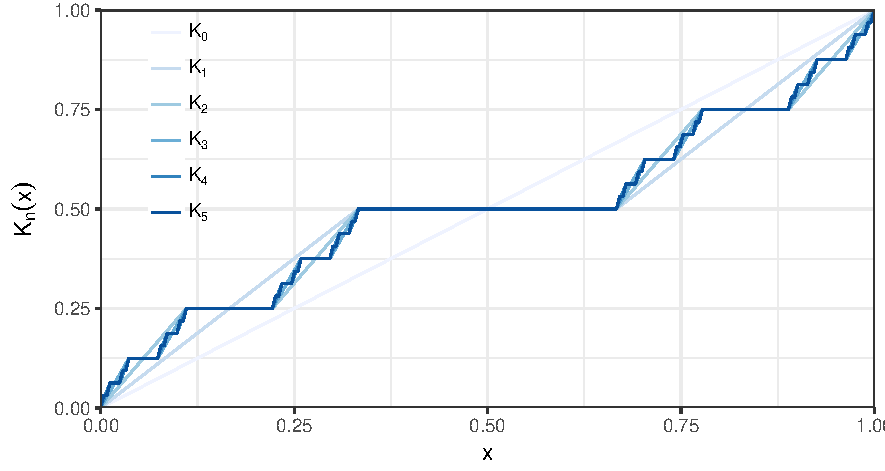
\includegraphics[width=\linewidth]{./img_mas_ejemplos/cantor.pdf}
\caption[Algunos pasos en la \textit{construcción iterativa} de la función de Cantor]{Algunos pasos en la \textit{construcción iterativa} de la función de Cantor, que es creciente, acotada y continua pero no absolutamente continua. En el texto, la función de Cantor es usado para construir medidas con propiedades patológicas.}
\end{figure}

%[?] demostracion de que la funcion de cantor esta bien definida
% https://es.wikipedia.org/wiki/Funci%C3%B3n_de_Cantor

\begin{proposicion}
La función de Cantor es continua pero no es absolutamente continua
\end{proposicion}

Luego entonces, puede construirse la siguiente función de distribución
\begin{equation}
F_K = \begin{cases}
K(x) &, 0\leq x \leq 1 \\
0 &, x < 0 \\
1 ,& x > 1
\end{cases}
\end{equation}
la cual no es ni continua ni discreta. Por simplicidad, en el presente trabajo únicamente se considerarán variables aleatorias que son continuas o discretas.

%La distinción entre variables aleatorias continuas y discretas puede verse más notoria en virtud del teorema \ref{Lebesgue_decomp}.

%\begin{teorema}[Descomposición de Radon-Nikodym]
%Sea $\mu$ una medida definida sobre la $\sigma$-álgebra $\mathcal{B}$, y sea $\nu$ una medida 
%$\sigma$-finita definida sobre $\mathcal{B}$. Entonces $\mu$ puede descomponerse de manera única como
%$\mu = \mu_A + \mu_S$, donde
%\begin{itemize}
%\item $\mu_A$ es absolutamente continua respecto a $\nu$
%\item Existe un conjunto $A$ tal que $\nu(A)=0$, $\mu_S\left(A^{C}\right) = 0$
%\end{itemize}
%\label{Lebesgue_decomp}
%\end{teorema}

%? pagina 109 del manual

%Dado que la medida de Lebesgue es $\sigma$-finita, cualquier medida de probabilidad puede 
%\textit{descomponerse} como la suma de una medida continua, una medida discreta y un \textit{residuo}.

\subsection{Valor esperado}

\begin{definicion}
Sea $X$ una variable aleatoria definida sobre el espacio de probabilidad $(\Omega, \mathcal{U}, P)$. Si $P$ es integrable en $\Omega$ respecto a $P$, entonces se define el \textbf{valor esperado} de $X$ como
\begin{equation}
\E{X} := \int_\omega X(\lambda) dP(\lambda)
\end{equation}
\end{definicion}

\begin{proposicion}
Sea $X$ una variable aleatoria y $g$ una función medible en el espacio medible $(\R,\mathcal{B})$. Entonces $g(X)$ es una variable aleatoria cuyo valor esperado es
\begin{equation}
\E{g(x)} = \int_\Omega [g(X)](\lambda) dP(\lambda) = \int_R g(x) dP(x)
\end{equation}
\end{proposicion}

\begin{definicion}
Sea $X$ una variable aleatoria, se definen su media $\mu_X$ y varianza $\sigma_X^{2}$ como
\begin{align}
\mu_X &{:=} \E{X} \\
\sigma_X^{2} &{:=} \E{(X-\mu_X)^{2}}
\end{align}
Por definición, no hay garantía que una variable aleatoria arbitraria tenga media o varianza bien definidas.
\end{definicion}

Naturalmente la notación $\mu_X$ únicamente se usa cuando no hay confusión con la notación para medidas. Así mismo, conviene mencionar ejemplos de variables aleatorias para las cuales no está bien definida su media o varianza.

? Ejemplos

%De manera más general, se define el $m$-momento de una variable aleatoria $X$ como
%\begin{equation}
%M
%\end{equation}

%\begin{definicion}
%Sea $X$ una varaible aleatoria. Se define su \textbf{función característica} como
%\begin{equation}
%\phi_X (\omega) := \E{e^{i \omega X}} = \int_\R e^{i \omega x} dF_X(x)
%\end{equation}
%donde, para todo $z\in \R$, $e^{i z} := \COS{z} + i \SEN{z}$
%\end{definicion}

\begin{definicion}
Sean $X$, $Y$ dos variables aleatorias. Se define su \textbf{covarianza} como
\begin{equation}
\Cov{X,Y} := \E{X Y} = \int_{\R^{2}} x y d P_{(X,Y)}(x,y) = \int_\R \int_\R x y dP_X(x) dP_Y(y)
\end{equation}
\end{definicion}

%\begin{proposicion}
%Si $X$, $Y$ son independientes, entonces $\Cov{X,Y} = 0$
%\end{proposicion}

\begin{definicion}
Sean $X$, $Y$ dos variables aleatorias. Se define su \textbf{coeficiente de correlación de Pearson} como
\begin{equation}
\rho (X,Y) := \sqrt{\frac{\Cov{X,Y}}{\Var{X} \Var{Y}}}
\end{equation}
\end{definicion}

%\begin{proof}
%en la pagina 65 del maual
%\end{proof}

\subsection{Vectores aleatorios}

El concepto de variable aleatoria real (definición ?) puede extenderse trivialmente a conjuntos más generales \textit{basados} en $\R$, como $\R^{n}$ para algún entero $n$; dicha generalización puede formalizarse fácilmente como otro caso particular.

\begin{definicion}
Se llama \textbf{vector aleatorio} a una variable aleatoria sobre el espacio de probabilidad $(\R^{n},\mathcal{B}^{n},P)$, para algún $n\in \N$. Se define a $\mathcal{B}^{n}$, la $\sigma$-álgebra de Borel $n$-dimensional, como
\begin{equation}
\mathcal{B}^{n} := \sigma\left(\left\{ \left(-\infty, a_1\right]\times \left(-\infty, a_2\right]\times \cdots \times \left(-\infty, a_n\right] \lvert a_1, \dots, a_n \in \R \right\}\right)
\end{equation}
\end{definicion}

Por notación, el vector aleatorio \textit{$n$-dimensional} $\boldsymbol{X}$ será referido como
\begin{equation}
\boldsymbol{X} = [X_1, X_2, \dots, X_n]
\end{equation}
esta notación para denotar vectores con \textit{símbolos gruesos} será usada durante el texto, extendida igualmente para realizaciones y otros vectores similares.

\begin{ejemplo}
Se dice que un vector aleatorio $\boldsymbol{X} = [X_1, X_2, \cdots, X_d]$ sigue una \textbf{distribución multinormal} si su función de probabilidad acumulada conjunta tiene la forma
\begin{equation}
F_{\boldsymbol{X}}\left( \boldsymbol{x} \right) = \frac{1}{\sqrt{(2\pi)^{d}\abso{C}}} \exp\left( -\frac{\boldsymbol{x} C^{-1} \boldsymbol{x}^{\intercal} }{2} \right)
\end{equation}
donde $\boldsymbol{x} = (x_1, x_2, \cdots, x_d)$. El vector $\mu \in \R^{d}$ será referido como \textit{vector de medias}, y la matriz $C \in \R^{d\times d}$ como \textit{matriz de covarianza}.
\end{ejemplo}

% si se necesita, esta en la pagina 30 del manual

%%%%%%%%%%%%%%%%%%%%%%%%%%%%%%%%%%%%%%%%%%%%%%%%%%%%%%%%%%%%%%%%%%%%%%%%%%%%%%%%%%%%%%%%%%%%%%%%%%%

\section{Estimación de parámetros}

Es común que se conozca cierta información de estos fenómenos que permita suponer que se comportan como variables aleatorias con cierta forma. Por ejemplo, ?.%se suele suponer que entre la población, 
%
Conviene destacar el caso de fenómenos que son \textit{forzados} a seguir una distribución conocida; por ejemplo, la metodología para aplicar la prueba Neuropsi \cite{Ostrosky00} ha sido diseñada de tal forma que los puntajes siguen una distribución normal para cada segmento poblacional.

En este tipo de escenarios se puede hablar de una función de distribución $f(\bullet; \theta)$ que depende de un parámetro $\theta \in \Omega$, donde $\Omega$ se conoce como \textbf{espacio de parámetros}; el objetivo consiste en deducir el valor de $\theta$ a partir de los datos recabados.

\begin{definicion}
Sea $X$ una variable aleatoria. Una \textbf{muestra de $X$ de tamaño $N$} es una colección de variables aleatorias $\{ X_1, X_2, \dots, X_N \}$ tales que son independientes y que comparten la misma distribución de $X$
\end{definicion}

\begin{proposicion}
Sea $X$ una variable aleatoria que admite una función de densidad $f_X$, y sea $\{ X_1, X_2, \dots, X_N \}$ una muestra. La función de densidad de probabilidad conjunta para el vector $[ X_1, X_2, \dots, X_N ]$ es
\begin{equation}
f_{[ X_1, \dots, X_N ]}(x_1, \dots, x_N ) = \prod_{j=1}^{N} f(x_j)
\end{equation}
Mientras no se indique lo contrario, las variables aleatorias en la muestra no están ordenadas.
\end{proposicion}

\begin{proposicion}
Sea $X$ una variable aleatoria, $\{ X_1, X_2, \dots, X_N \}$ una muestra y $\{ x_1, x_2, \dots, x_N \}$ un conjunto de observaciones. Se define la \textbf{función de distribución muestral} como
\begin{equation}
F_{X; N} (x) := \frac{1}{N} \sum_{x_j \leq x } 1
\end{equation}
\end{proposicion}

\begin{proposicion}
Si el tamaño de una muestra de $X$ se vuelve arbitrariamente grande, la función de distribución muestral converge en probabilidad a $F$, la función de probabilidad acumulada de $X$
\begin{equation}
\lim_{N \rightarrow \infty} F_{X; N} = F_X
\end{equation}
\end{proposicion}

%\begin{proof}
%Ver seccion 5.2 C R Rao, Linear Statistic Inference and its applications 2 ed pag 42
%\end{proof}

\begin{definicion}
Un \textbf{estadístico} es una función de las observaciones en una muestra
\end{definicion}

Ejemplo en pagina 112 del libro de lindgren.
Si $X\sim N(\mu,\sigma^{2})$, sea $\overline{X} = \frac{1}{N} \sum X_j$, entonces
\begin{equation}
\overline{X} \sim N(\mu,\frac{\sigma^{2}}{N})
\end{equation}

\begin{teorema}[Cramér-Rao]
Sea $\widehat{\theta}$ un estimador insesgado de $\theta$. Si la función de verosimilitud asociada al estimador, $L$, es diferenciable, entonces
\begin{equation}
\Var{\widehat{\theta}} \geq \left( \E{\frac{\partial}{\partial\theta} L(X; \theta)} \right)^{-2}
\end{equation}
La igualdad se alcanza si y sólo si existe una función positiva $k$ tal que puede escribirse
\begin{equation}
\frac{\partial}{\partial\theta} L(X; \theta) = k(\theta) \left[ \widehat{\theta}(X) - \theta \right] 
\end{equation}
\end{teorema}


%Ejemplo.
%Considérese la variable aleatoria binomial $X \sim B(\theta)$ con $\theta \in [0, 1]$, cuya FDP es
%\begin{equation}
%f_X(x; \theta) = \begin{cases}
%\theta^{x} (1-\theta)^{1-x} &, x\in \{ 0,1 \} \\
%0 &, \text{otro caso}
%\end{cases}
%\end{equation}
%La FDP conjunta para una muestra de tamaño $N$ es
%\begin{equation}
%f_N(x_1, \dots, x_N; \theta) = 
%\begin{cases}
%\theta^{\sum_i x_i}(1-\theta)^{\sum_i(1-x_i)} &, x_i \in \{ 0,1 \}, i\in \{1, \dots, N\} \\
%0 &, \text{otro caso}
%\end{cases}
%\end{equation}
%
%Se puede entender a $f_N$, evaluada en los datos obtenidos y como función de $\theta$, como la probabilidad de que se hayan obtenido los datos que de hecho se obtuvieron.
%%
%Esta redundancia sugiere que una elección adecuada para el parámetro $\theta$ sería aquél que maximice a tal función, que que recibe el nombre de \textbf{función de verosimilitud}
%\begin{equation}
%L(\theta; x_1, \dots, x_N) = \theta^{\sum_i x_i}(1-\theta)^{\sum_i(1-x_i)}
%\end{equation}
%con $\theta \in [0, 1]$. Por simplicidad técnica, se maximizará a $L$ igualando a cero la derivada de $\log \circ L$ con respecto a $\theta$.
%\begin{align*}
%\frac{d}{d\theta} \log\left( L(\theta; x_1, \dots, x_N)\right)
%&= 
%\frac{d}{d\theta} \log\left(\theta^{\sum_1^{N} x_i}(1-\theta)^{\sum_1^{N}(1-x_i)}\right) \\
%&=
%\frac{d}{d\theta} \left[ \left( \sum_{1}^{N} x_i \right) \log(\theta) + 
%\left( \sum_{1}^{N}(1-x_i) \right) \log (1-\theta)\right] \\
%&= \left( \sum_{i=1}^{N} x_i \right) \frac{1}{\theta} -
%\left( N - \sum_{i=1}^{N}(x_i) \right) \frac{1}{1-\theta}
%\end{align*}
%
%Luego entonces, la función de verosimilitud es maximizada usando $\theta = \frac{1}{N} \sum_{1}^{N}(x_i)$.

\begin{definicion}
Sea $X$ una variable aleatoria que depende de un parámetro $\theta$ y $X_1, \dots, X_N$ una muestra de tamaño $N$. Un estimador $\widehat{\theta}$ es \textbf{suficiente} si
la distribución de la variable $X \lvert \widehat{\theta}$ no depende de $\theta$
\end{definicion}

\begin{teorema}
Sea $X$ una variable aleatoria que depende del parámetro $\theta$. Un estadístico $\widehat{\theta}$ es suficiente si y sólo si existen funciones $g$ y $h$ tales que
\begin{equation}
f_X(\bullet; \theta ) = g(\widehat{\theta},\theta) h_X(\bullet)
\end{equation}
\end{teorema}

%\begin{proof}
%ver pagina 121 del libro de lindgren
%\end{proof}

%El \textbf{espacio de datos} es 

%Usando la desigualdad de Chebyshev de puede deducir que
%\begin{equation}
%P\left( \abso{\widehat{\theta} - \theta} > \varepsilon \right) \leq 
%\frac{1}{\varepsilon^{2}} \E{\left( \widehat{\theta} - \theta \right)^{2}}
%\end{equation}

\begin{definicion}
El \textbf{error de media cuadrática} para el estimador $\widehat{\theta}$ se define como
\begin{equation}
\text{EMC}(\widehat{\theta}) := \E{\left( \widehat{\theta} - \theta \right)^{2}} =
\Var{\widehat{\theta}} + \left( \E{\theta} - \theta^{2} \right)
\end{equation}
\end{definicion}

\begin{definicion}
Sea $X$ una variable aleatoria que depende de un parámetro $\theta$ y $X_1, \dots, X_N$ una muestra de tamaño $N$. Un estimador $\widehat{\theta}$ es \textbf{insesgado} si cumple que
\begin{equation}
\E{\widehat{\theta}} = \theta
\end{equation}
\end{definicion}

Se puede hablar del \textbf{sesgo} del estimador $\widehat{\theta}$ como $\E{\widehat{\theta}}-\theta$

\begin{definicion}
Sea $X$ una variable aleatoria que depende de un parámetro $\theta$ y $\left\{ \widehat{\theta}_n \right\}_{n\in \N}$ una familia de estimadores definidos para muestras de $X$ de tamaño arbitrario. La familia de estimadores se dice \textbf{consistente} si para cualquier $\varepsilon > 0$
\begin{equation}
\lim_{n\rightarrow\infty} P\left( \abso{\widehat{\theta}_n-\theta} > \varepsilon \right) = 0
\end{equation}
\end{definicion}

\begin{definicion}
Así como en la definición anterior, se dice que a familia de estimadores \textit{converge en media cuadrática} si
\begin{equation}
\lim_{n\rightarrow\infty} \E{\left( \widehat{\theta}_n - \theta \right)^{2}} = 0
\end{equation}
Si esto se cumple, se dice que la familia de estimadores es \textbf{consistente en media cuadrática} \end{definicion}

\begin{proposicion}
Si $\widehat{\theta}_n$ es una familia de estimadores consistente en media cuadrática, entonces es consistente
\end{proposicion}

\begin{proposicion} COROLARIO
Una condición suficiente para para que una familia sea consistente en en media cuadrática es
\begin{align}
\lim_{n\rightarrow\infty} \E{\widehat{\theta}_n} &= \theta \\
\lim_{n\rightarrow\infty} \Var{\widehat{\theta}_n} &= 0
\end{align}
\end{proposicion}

%\begin{proof}
%? pag 141 del libro de lindgren
%\end{proof}

\begin{teorema}[Límite central]
Sea $\{ X_1, \cdots, X_N\}$ una muestra de tamaño $N$ de una variable aleatoria con distribución normal, $X\sim N(\mu,\sigma^{2})$. Defínase la variable aleatoria $Y_N$ como
\begin{equation}
Y_N = \frac{\sum_{i=1}^{N}X_i - N \mu}{\sqrt{N \sigma^{2}}}
\end{equation}
Entonces $\{ Y_N \}_{N \in \N}$ converge en probabilidad a una distribución normal $N(0,1)$.
\end{teorema}


%%%%%%%%%%%%%%%%%%%%%%%%%%%%%%%%%%%%%%%%%%%%%%%%%%%%%%%%%%%%%%%%%%%%%%%%%%%%%%%%%%%%%%%%%%%%%%%%%%%

\section{Procesos estocásticos}

Los procesos estocásticos se definen formalmente como variables aleatorias cuyo espacio muestral es un espacio de funciones.
%, para lo cual deben definirse previamente una $\sigma$-álgebra \textit{suficientemente buena} para estos espacios.
%
Intuitivamente es posible definir %(alternativamente) 
los procesos estocásticos como una \textit{concatenación} de variables aleatorias, es decir, un conjunto de variables aleatorias indexadas sobre algún conjunto arbitrario.
%
Sin embargo, indexar un conjunto infinito de variables aleatorias representa un problema técnico en el cuanto a definir al proceoso estocástico como espacio de probabilidad, especialmente al definir la medida de probabilidad asociada.

Debido a las limitaciones del presente trabajo, el tema se expone de manera parcial bajo un enfoque formal; la exposición se basa en aquella presentada por [Kolmogorov?], de modo que el lector interesado debe dirigirse a dicho texto.

Primeramente se define a $\R^{\mathcal{T}}$, el conjunto de funciones con dominio en $\mathcal{T}$ y codominio en $\R$, el cual será usado como espacio de eventos\footnote{Se puede definir análogamente a $\C^{\mathcal{T}}$, o espacios más generales}. 
%
A modo de \textit{intervalos generalizados} se definen los conjuntos de la forma
\begin{equation}
I\left( [t_1, a_1, b_1], \cdots, [t_N, a_N, b_N] \right) = 
\left\{ f \in \R^{\mathcal{T}} \talque f(t_i) \in (a_i, b_i] \, , \, i = 1, \cdots, N \right\}
\end{equation}

Es relativamente fácil extender la familia de estos intervalos por uniones e intersecciones finitas. Es un tanto más interesante definir una $\sigma$-álgebra generada por éstos conjuntos, pero tal parte se omite en el presente trabajo.
%
En el texto por Kolmogorov se explora con mayor detalle la existencia de dicha $\sigma$-álgebra --y por tanto, la existencia de procesos estocásticos.

\begin{definicion}
Un \textbf{proceso estocástico} \xt es una colección de variables aleatorias indexadas por el símbolo $t\in\mathcal{T}$.
%\begin{equation}
%\{X(t)\}_{t\in \mathcal{T}} := \left\{ X(t) \lvert t\in \mathcal{T} \right\}
%\end{equation}
\end{definicion}

\begin{definicion}
Se dice que un proceso estocástico \xt es un \textbf{proceso estocástico en $\R$} si cumple que $\mathcal{T} \subseteq \R$.
%
Por notación, el índice $t$ es referido como \textbf{tiempo}, mientras que $\mathcal{T}$ es el conjunto de \textbf{tiempos admisibles}.
\end{definicion}

Por simplicidad, durante el presente trabajo sólo se usarán dos familias de procesos estocásticos en $\R$: si $\mathcal{T}$ es un intervalo, o si es parte de una \textit{malla}. 
%
La primera familia se reserva para modelar las señales electrofisiológicas, mientras que la segunda se usará para modelar los registros de estas mismas señales.
%
La distinción consiste en que las señales electrofisiológicas sólo pueden ser registradas digitalmente en un conjunto finito de puntos en el tiempo; la atención del texto recae en ambos grupos de procesos, en espera que sus características sean similares de algún modo.

\begin{definicion}
Se dice que un proceso estocástico en $\R$ es \textbf{a tiempo continuo} si existen $a, b \in \R \cup \{ -\infty, \infty \}$ tales que
\begin{equation}
\mathcal{T} = (a,b)
\end{equation}
Así mismo, se dice que un proceso estocástico en $\R$ es \textbf{a tiempo discreto} si existen $t_0, \Delta_X \in \R \cup \{ -\infty, \infty \}$ tales que
\begin{equation}
\mathcal{T} = \left\{ t_0 + t \in \R \talque {t} \cdot {\Delta_X} \in \Z \right\}
\end{equation}
Por notación, $\Delta_X$ es referida como \textit{frecuencia de muestreo}.
\end{definicion}

Conviene destacar que el nombre \textit{frecuencia de muestreo} hace referencia al proceso de registro, que algunos textos es referido como \textit{muestreo}; esta terminología entra claramente en conflicto con las muestras de una variable aleatoria. En lo siguiente se evita llamar muestreo al proceso de registro, pero se conservará el término frecuencia de muestro.

Cabe mencionar que hay un conflicto similar con los términos \textit{tiempo continuo} y \textit{tiempo discreto}; estos términos \underline{no guardan ninguna analogía} con las variables aleatorias discretas y continuas, ni con los espectro de potencias puramente continuos o puramente discretos (ver el capítulo siguiente).
%
Estos términos se usan porque se encuentran muy extendidos en la literatura sobre análisis de señales.

Para facilitar la referencia de procesos estocásticos, los elementos que lo componen son denotados como:
\begin{tabular}{cl}
\xt    & Todo el proceso \\
$X(t)$ & Variable aleatoria en el proceso, para el tiempo $t$ \\
$x(t)$ & Una realización de $X(t)$ \\
$F_{X(t)}$ & Función de probabilidad acumulada para $X(t)$
%$ {\Delta_t}$ & Frecuencia de muestreo (en tiempo discreto)
\end{tabular}

%Una primera función asociada a los procesos estocásticos es la autocorrelación.

\subsection{Estacionariedad débil}

De forma general, la estacionariedad significa que \textit{algunas} propiedades de un proceso sean \textit{invariantes} en el tiempo; la decisión sobre qué características deben ser invariantes, y en qué sentido, conlleva a diferentes definiciones.
%
Por ejemplo, en la definición \ref{est_fuerte} se pide que todas las variables que integra al proceso sigan una distribución común, así como todas variables conjuntas con algunas características.

%La estacionariedad es un indicativo de la \textit{homogeneidad} de un proceso; un proceso 
%\textit{muy} estacionario sería aquél cuyas variable aleatoria que tiene distribuciones conjuntas que no cambian 
%con el tiempo. 
%%
%La definición \ref{est_fuerte} representa con exactitud tales requerimientos, pero se le considera 
%\textit{innecesariamente fuerte}; una definición común es \ref{est_m}.

\begin{definicion}%[Estacionariedad fuerte]
Un proceso \xt se dice \textbf{fuertemente estacionario} si para cualesquiera $t_1, t_2, \dots, t_n \in \mathcal{T}$ y cualquier $\tau$ tal que $t_i + \tau \in \mathcal{T}$, se cumple que
\begin{equation*}
F_{\left[ X(t_1), X(t_2), \dots, X(t_n) \right]} \equiv
F_{\left[ X(t_1 + \tau), X(t_2 + \tau), \dots, X(t_n + \tau) \right]}
\end{equation*}
con $F_{[v_1,v_2,\dots,v_N]}$ es la función de probabilidad acumulada para el vector $[v_1,v_2,\dots,v_N]$.
\label{est_fuerte}
\end{definicion}

En el contexto del presente trabajo la estacionariedad fuerte se considera \textit{innecesariamente fuerte}, en cuanto a que es difícil de verificar y porque se usarán hipótesis más débiles.
%
Se decidió conveniente una definición que garantice que los momentos puedan ser estimados, para lo cual deben ser constantes en el tiempo.
%
La motivación principal para ello es el siguiente: si se modela una señal como proceso estocástico, entonces los momentos están asociados con variables físicas relevantes. 
%
En particular, el segundo momento está asociado con la \textit{energía} (ver ??).

\begin{definicion}%[Estacionariedad de orden $m$]
Un proceso \xt se dice \textbf{estacionario de orden $\boldsymbol{m}$} si, para cualesquiera $t_1, t_2, \dots, t_n \in \mathcal{T}$ y cualquier $\tau$ tal que $t_i + \tau \in \mathcal{T}$, se cumple que
\begin{equation*}
\E{X^{m_1}(t_1)X^{m_2}(t_2)\cdots X^{m_n}(t_n)} =
\E{X^{m_1}(t_1+\tau)X^{m_2}(t_2+\tau)\cdots X^{m_n}(t_n+\tau)}
\end{equation*}
para cualesquiera enteros $m_1, m_2, \dots, m_n$ tales que $m_1+m_2+\cdots+m_n \leq m$.
\label{est_m}
\end{definicion}

%Cabe mencionar que la definición \ref{est_m} no es equivalente a la definición \ref{est_fuerte}, ni
%aún cuando $m\rightarrow \infty$; sin embargo permite asegurar que los \textit{momentos} 
%($\E{X^{k}}$ para algún $k$) del proceso sean invariantes en el tiempo, y éstos suelen encontrarse
%asociados a cantidades físicas.

La definición \ref{est_m} es conveniente tomando en cuenta que para estudiar la energía de un proceso (asociada al segundo momento) requerirá poner condiciones adicionales; por ejemplo, para estimar la varianza de la energía en un proceso, a partir de observaciones, se requiere que el proceso sea estacionario de orden 4.
%
En el otro sentido, siempre que sea posible se usará la menor cantidad de hipótesis, para lo cual se presenta una definición más particular y \textit{débil} de estacionariedad.

%Como un ejemplo muy particular conviene destacar la energía, que suele ser asociada con el segundo
%momento (definición \ref{energia}). 
%%
%Dicha conexión motiva a escoger una definición de estacionariedad que permita analizar la energía 
%del proceso: la estacionariedad débil.

\begin{definicion}%[Estacionariedad débil]
Un proceso \xt se dice \textbf{débilmente estacionario} si existen constantes $\mu, \sigma \in \R$ y una función $R : \mathcal{T} \rightarrow \R \cup \{ \pm \infty \} $ tales que, para cualesquiera $t, s \in T$ se 
cumple
\begin{itemize}
\item $\E{X(t)} = \mu$
\item $\Var{X(t)} = \sigma^{2}$
\item $\Cov{X(t),X(s)} = R(\abso{s-t})$
\end{itemize}
\end{definicion}

\begin{proposicion}
Para que un proceso estocástico \xt sea débilmente estacionario es suficiente y necesario que sea estacionario de orden 2.
\end{proposicion}

%\begin{proof}
%\underline{Para probar que la condición es necesaria} supóngase que \xt es débilmente estacionario.
%Para que sea estacionario de orden 2 debe cumplirse que, para cualesquiera $s, t, s+\tau, y+\tau \in \mathcal{T}$
%\begin{enumerate}
%\item $\E{X(t)} = \E{X(t+\tau)}$
%\item $\E{X^{2}(t)} = \E{X^{2}(t+\tau)}$
%\item $\E{X(t)X(s)} = \E{X(t+\tau)X(s+\tau)}$
%\end{enumerate}
%
%\underline{Para probar que la condición es necesaria} supóngase que \xt es estacionario de orden 2.
%%
%Se toma un $t_0\in \mathcal{T}$ arbitrario, y se define
%\begin{equation*}
%\mu = \E{X(t_0)} \qquad \sigma^{2} = \Var{X(t_0)}
%\end{equation*}
%\end{proof}

El que un proceso sea débilmente estacionario implica la existencia de una media y varianza características del proceso, es decir, que son comunes a todas las variables aleatorias que lo componen. 
%
Además, se implica la existencia de una función referida como \textit{autocovarianza}.

\begin{definicion}
Sea \xt un proceso estocástico sobre $\R$. Su \textbf{función de autocovarianza} es una función $R: \R^{2}\rightarrow \R$ tal que
\begin{equation}
R(t,s) = \E{\left(X(t) - \E{X(t)}\right)\overline{\left(X(s) - \E{X(s)}\right)}}
\end{equation} 
para cualesquiera tiempos admisibles $s, t \in \mathcal{T}$.
\end{definicion}

\begin{figure}
\centering
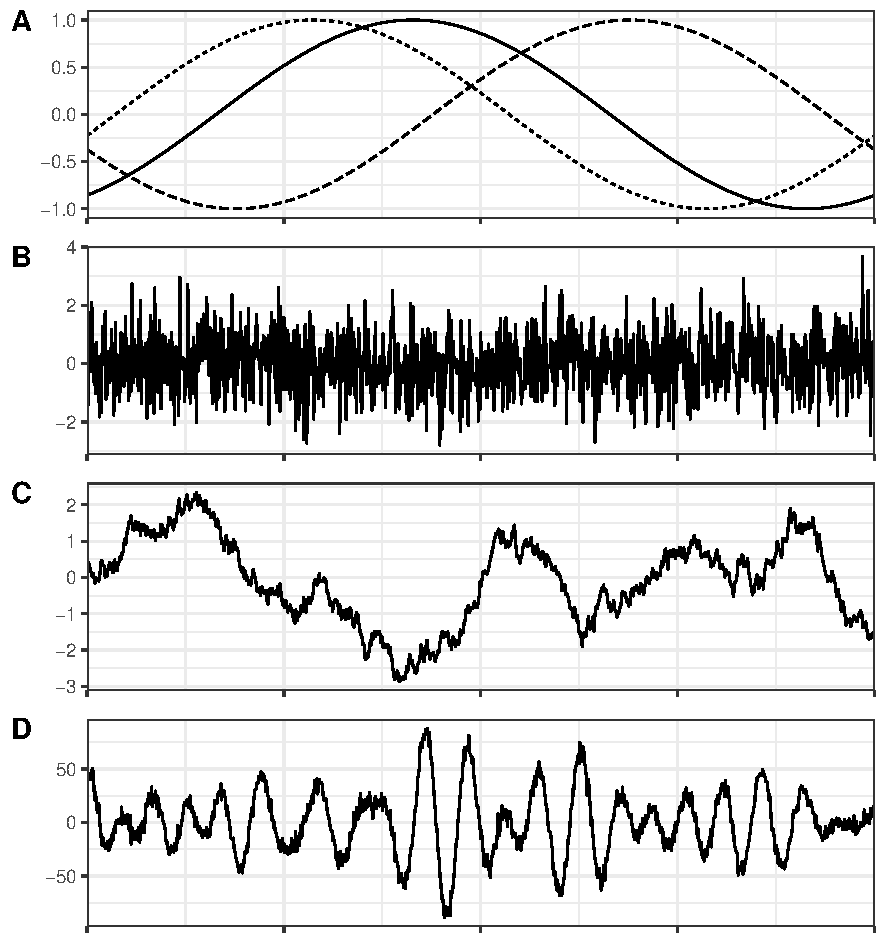
\includegraphics[width=\linewidth]{./img_mas_ejemplos/ruidos_ejemplos.pdf}
\caption[Ejemplos de procesos débilmente estacionarios]{Ejemplos de procesos débilmente estacionarios. \textbf{A.} Proceso oscilante, del cual se grafican tres realizaciones diferentes. \textbf{B.} Proceso Ruido Blanco. \textbf{C.} Proceso de medias móviles (MA). \textbf{D.} Proceso tipo alfa. }
\end{figure}

%La proposición anterior deja en claro que la estacionariedad débil puede entenderse como una \textit{estabilidad} en los momentos conjuntos de orden al menos dos, condición suficiente para trabajar con la media y la varianza del proceso.
%
%Sin embargo, en ocasiones se requerirán condiciones más fuertes sobre los procesos. Como ejemplo, cuando se quiere obtener la varianza para un estimador del espectro de potencias, se necesita que la serie sea estacionaria de orden 4. 

%Cabe destacar que la estacionariedad débil no sólo tiene como condición que todas las variables del
%proceso tengan la misma media y varianza, sino que también supone que éstas son finitas.
%
%Sobre la función de covarianza $R$ (que en un único proceso es referida como \textit{autocovarianza}),
%no hay restricciones sobre los valores que pueda tomar, excepto que 
%$R(0) = \Var{X(\bullet)} < \infty$. 

Como las señales electrofisiológicas son modeladas como procesos estocásticos, conviene traducir algunas de sus características en propiedades para los procesos estocásticos.
%
Por ejemplo, se sabe que las señales representan variaciones en campos eléctricos, y entonces se puede afirmar sin duda que dicha cantidad es finita en todo momento; lo mismo se puede afirmar sobre la energía.
%
En base a ello, los procesos estocásticos que modelan señales electrofisiológicas deben tener energía y varianza finitas en todo momento.
%
%En el marco del modelo de series electrofisiológicas, conviene suponer que los registros 
%corresponden a procesos a tiempo continuo que son continuos de alguna forma; se ha elegido la 
%continuidad en media cuadrática.
%
%Cuando una señal electrofisiológica se modela como un proceso estocástico, es necesario suponer que su media y varianza son finitas en todo momento. 
%
%Esto se debe a que existen umbrales \textit{naturales} en los que ocurren las mediciones, fuera de los cuales la vida misma es imposible; este comentario aplica también sobre la energía dentro del sistema.
%
Más aún, la actividad eléctrica cerebral y muscular presentan durante el reposo una actividad característica, referida como \textit{actividad basal} o \textit{línea base}, que es relativamente cercana a una constante en todo momento (ver figura \ref{ejemplos_mor}).
%; esta actividad es 
%) de la cual no se \textit{alejan mucho}.
%el resto del tiempo
%La línea base es aproximadamente una línea recta
%Esta suerte de media intuitiva es referida como \textit{línea base}, y se refleja dentro del modelado con la insistencia heurística de tratar a los procesos como si tuvieran media cero.
%
El fenómeno de línea base entra en el modelado como el supuesto de que las señales son procesos estacionarias de orden 1; por simplicidad, se puede considerar que la media de estos procesos es 0.

Una segunda característica de las señales que se traduce es la continuidad: las señales representan fenómenos eléctricos que cambian de manera \textit{suave} en el tiempo, e idealmente son curvas derivables.
%
El aspecto de los registros con \textit{picos} se explica porque el cambio es suave, pero es muy rápido respecto a la tasa de registro.

\begin{proposicion}
Sea \xt un proceso débilmente estacionario y $R$ su función de autocovarianza. Si $R$ es continua
en 0 entonces es continua en todo $\R$.
\end{proposicion}

\begin{proof}
Supóngase que $R$ es continua en 0. Tómese a $t_0 \in \mathcal{T}$ arbitrario para verificar que $R$ es continua en $t_0$, y tómense $s,h$ tales que $s,s+t,s+t+h \in\mathcal{T}$. Usando la desigualdad de Schwarz, puede escribirse que
\begin{align*}
\left[ R(t_0+h) -R(t_0) \right]^{2} 
&= \left( \E{X(s+t_0+h)X(s)} - \E{X(s+t_0)X(s)} \right)^{2}  \\
&= \left( \E{X(s)\left[ X(s+t_0+h) - X(s+t_0) \right]} \right)^{2} \\
&\leq \E{\left( X(s) \right)^{2}} \E{\left( X(s+t_0+h) - X(s+t_0) \right)^{2}} \\
&\leq 2 \sigma_X^{2} \left[ \sigma_X^{2} - R(h) \right]
\end{align*}
%&\leq \sigma_X^{2} \left[ \Var{X(s+t_0+h)} + \Var{X(s+t_0)} - 2 \Cov{X(s+t_0+h), X(s+t_0)} \\
Entonces, puede afirmarse que
\begin{equation*}
\abso{R(t_0+h) -R(t_0)} \leq \sqrt{2 \sigma_X^{2}} \sqrt{R(0) - R(h)}
\end{equation*}
Como $R$ es continua en 0, entonces 
\begin{align*}
\lim_{h\rightarrow 0} (R(0)-R(h)) = 0 &\Rightarrow \lim_{h\rightarrow 0} (R(t_0+h)-R(t_0)) = 0
\end{align*}
de donde se concluye que $R$ es continua en $t_0$, para cualquier $t_0\in \mathcal{T}$.
\end{proof}    

\begin{definicion}%[Continuidad estocástica en media cuadrática]
Un proceso a tiempo continuo \xt se dice \textbf{estocásticamente continuo, en el sentido de media cuadrática}, en el tiempo $t_0\in \mathcal{T}$ si
\begin{equation*}
\lim_{t \rightarrow t_0} \E{\left( X(t) - X(t_0) \right)^{2}} = 0
\end{equation*}
\label{cont_est}
\end{definicion}

Por simplicidad, y porque es la única definición de su tipo usada en el presente trabajo, la continuidad estocástica en media cuadrática será referida simplemente como \textit{continuidad estocástica}.

%Una forma natural de pensar en la definición \ref{cont_est} es que si $\abso{t-t_0}$ es muy pequeño 
%entonces $X(t)$ y $X(t_0)$ difieren muy poco entre sí, como variables aleatorias.
%%
%Hablando de procesos débilmente estacionarios, la continuidad estocástica de un proceso es 
%equivalente a que su función de autocovarianza sea continua en 0.

\begin{proposicion}
Sea \xt un proceso a tiempo continuo, débilmente estacionario y de media cero, y sea $R$ su función de autocovarianza. El proceso es estocásticamente continuo en $t_0\in \mathcal{T}$ si y sólo si $R$ es continua en $0$.
\end{proposicion}

\begin{proof}
Para cualquier $t\in \mathcal{T}$, puede escribirse
\begin{align*}
\E{\left( X(t) - X(t_0) \right)^{2}} &= \Var{X(t)} + \Var{X(t_0)} - 2 \Cov{X(t),X(t_0)} \\
&= 2 \left( \sigma_X^{2} - R(t-t_0) \right) \\
&= 2 \left( R(0) - R(t-t_0) \right)
\end{align*}
Así entonces, la condición para continuidad estocástica puede reescribirse como
\begin{align*}
\lim_{t \rightarrow t_0} \E{\left( X(t) - X(t_0) \right)^{2}} = 0 
&\Leftrightarrow
\lim_{t \rightarrow t_0} \left( R(0) - R(t-t_0) \right) = 0 \\
&\Leftrightarrow
\lim_{\tau \rightarrow 0} R(\tau) = R(0)
\end{align*}
\end{proof}

\begin{definicion}
Se dice que una función $f: \R\rightarrow \R$ es \textbf{definida positiva} si para cualesquiera $x_1, _2, \cdots, x_N \in \R$, $z_1, z_2, \cdots, z_N \in \R$ se cumple que 
\begin{equation}
\sum_{n=1}^{N} \sum_{m=1}^{N} z_n z_m f(x_m-x_n) \leq 0
\end{equation}
\end{definicion}

\begin{proposicion}
Sea \xt un proceso débilmente estacionario y $R$ su función de autocorrelación. Se cumple que $R$ es una función positiva definida.
\end{proposicion}

\begin{proof}
Sean $t_1, t_2, \cdots, t_N \in \mathcal{T}$, $z_1, z_2, \cdots, z_N \in \R$ arbitrarios. Se construye la variable aleatoria $W$ como
\begin{equation}
W = \sum_{n=1}^{N} z_n X(t_n)
\end{equation}

Ahora, nótese que
\begin{align*}
0 &\leq \Var{W} \\
&= \sum_{m=1}^{N} \sum_{n=1}^{N} z_m z_n \Cov{X(t_m),X(t_n)} \\
&= \sum_{m=1}^{N} \sum_{n=1}^{N} z_m z_n R(t_m-t_n)
\end{align*}
\end{proof}

%%%%%%%%%%%%%%%%%%%%%%%%%%%%%%%%%%%%%%%%%%%%%%%%%%%%%%%%%%%%%%%%%%%%%%%%%%%%%%%%%%%%%%%%%%%%%%%%%%%

\section{Pruebas de hipótesis}

%? empieza en la pagina 156 del libro de lindgren

Una hipótesis es una afirmación sobre algún aspecto desconocido.
%
Es tarea común en la estadística el decidir si alguna afirmación puede sostenerse a partir de la
información proporcionada por un conjunto de observaciones. 
%
A partir de la aplicación masiva de pruebas neuropsicológicas a un grupo de adultos mayores uno 
puede preguntarse, por ejemplo, si hombres y mujeres tienden a obtener puntajes diferentes en las
pruebas, o si la edad de los participantes está correlacionada con su desempeño en tareas de 
memoria.
%
En la tabla ... se muestran los datos sobre una simulación (artificial) de dicho escenario.

Una herramienta de uso común para producir estas decisiones es la \textbf{pruebas de hipótesis},
la cual consiste en dos afirmaciones complementarias, es decir, tales que exactamente una de ellas es verdadera; tales afirmaciones
son referidas como \textit{hipótesis}, y deben elegirse de forma que sean equivalentes a la 
decisión que se busca. 
%
Usualmente la primera de las hipótesis (hipótesis nula, $H_0$) representa la afirmación más general o que se cree verdadera por omisión, mientras que la segunda hipótesis (hipótesis alternativa, $H_A$) se tomará como verdadera si
existe suficente información para rechazar la veracidad de la primera.
%
%La idea intuitiva detrás de las pruebas estadísticas es que una muestra de la población se comporta de manera similar a la población.
%
El enfoque de prueba de significancia es  tomar un estadístico $\est{\theta}$ y evaluarlo sobre los datos, posteriormente se analiza qué tan diferente es el valor obrevado del típico cuando la hipótesis nula es verdadera.

Los estadísticos de prueba suele ser un estadístico construido para tener una distribución conocida salvo unos pocos parámetros fáciles de estimar.
%
La interpretación usual es que, si $H_0$ es verdadera entonces $\est{\theta}$ puede no tener el valor predicho debido a factores ajenos al fenómeno estudiado, en consecuencia se suele hablar de una región de rechazo en el espacio de estados (ver más adelante).
%
Bajo esta interpretación, un valor de $\widehat{\theta}$ dentro de la región de rechazo significa que los datos representan evidencia para rechazar $H_0$; un no-rechazo no significa precisamente que $H_0$ sea verdadera, sino que las observaciones no representan evidencia suficiente para rechazar $H_0$.

\begin{definicion}
En una prueba de hipótesis, rechazar $H_0$ cuando es verdadero es un \textbf{error del tipo I}. Así msimo, aceptar $H_0$ cuando es falsa es un \textbf{error del tipo II}.
\end{definicion}

La naturaleza e intepretación de los estadísticos de prueba suelen ser muy particulares de las situaciones bajo las cuales son definidos.
%
Una forma típica de normalizar los diferentes estadísticos es a través del $p$-valor, definido como la probabilidad de que ocurra un valor extremo del estadístico de prueba; 
el $p$-valor suele interpretarse como la \textit{fuerza} de la evidencia contra $H_0$.

\begin{definicion}
Sea $\widehat{\theta}$ un estadístico de prueba. El \textbf{$\boldsymbol{p}$-valor} asociado al $\widehat{\theta}=\theta_0$ es la probabilidad $P\left(\widehat{\theta}\right>\theta_0)$
\end{definicion}

Una \textbf{prueba de sinificancia} se entiende como una pruebas de hipótesis para algunos $p$-valores predefinidos, usualmente 0.05, 0.01, 0.005, entre otros.
%
Un error común, pero muy extendido, es interpretar al $p$-valor como la probabilidad de obtener $H_0$.

\begin{definicion}
Dada una muestra poblacional y dos afirmaciones complementarias $H_0$ y $H_A$, una \textbf{prueba de hipótesis} es una regla de decisión que asigna a cada punto del espacio de estados una acción del conjunto Aceptar $H_0$, rechazar $H_A$, Rechazar $H_0$, aceptar $H_A$.

Al conjunto del espacio muestral sonde se rechaza $H_0$ se le denomina \textbf{región crítica}. 
\end{definicion}

%\begin{definicion}
%La función de potencia es el supremo, sobre todas las distribuciones muestrales, de la probabilidad de que una muestra
%\end{definicion}

%Por comodidad, uno puede redefinir a la región crítica en términos del estimador $\widehat{\theta}$. 
Una propiedad deseable para un estadístico de prueba es poder acotar los errores de tipo I y de tipo II; para ello, para alguna región crítica arbitraria $\mathcal{C}$ se define el \textbf{nivel de significancia} de la prueba como
\begin{equation}
\alpha := \sup_{\theta \in H_0} p(\mathcal{C} \lvert \theta)
\end{equation}

Ejemplo:
Retomando los datos de la tabla ..., considérese la pregunta \textit{¿Los hombres y mujeres tienden
a obtener puntajes diferentes en las pruebas neuropsicológicas?}. 
%
En este ejemplo se supone que los puntajes de los hombres en la prueba siguen una distribución normal con media $\mu_H$ y varianza 1, y similarmente para las mujeres con media $\mu_M$ y varianza 1.
%
Como hipótesis nula se elige la posibilidad de que en promedio ambos grupos (hombre y mujeres) obtengan el mismo puntaje en la prueba, es decir
\begin{equation}
H_0 : \mu_H = \mu_M
\end{equation}
y como hipótesis alternativa está la posibilidad de que los puntajes sean diferentes
\begin{equation}
H_A : \mu_H \neq \mu_M
\end{equation}

%\subsection{Clasificación de dos vías}
%
%Un \textbf{diseño aleatorio por bloques} es un muestreo aleatorio en varias categorías de sujetos 

%%%%%%%%%%%%%%%%%%%%%%%%%%%%%%%%%%%%%%%%%%%%%%%%%%%%%%%%%%%%%%%%%%%%%%%%%%%%%%%%%%%%%%%%%%%%%%%%%%%
%%%%%%%%%%%%%%%%%%%%%%%%%%%%%%%%%%%%%%%%%%%%%%%%%%%%%%%%%%%%%%%%%%%%%%%%%%%%%%%%%%%%%%%%%%%%%%%%%%%

\section{Espacios de Hilbert}

A grosso modo, un espacios de Hilbert es un conjunto de \textit{vectores} en donde se ha definido un producto de vectores, el cual induce una métrica según la cual todas las sucesiones de vectores convergen.
%
Es una estructura tan general que puede ser \textit{inducida} sobre una gran variedad de conjuntos, tal como se hace en el siguiente capítulo.

Para poder definir adecuadamente estos objetos hay que definir, en ese orden, los siguientes conceptos: campo, espacio vectorial, producto interno, norma, métrica.
%
Debido a los fines de este trabajo, se da una clara preferencia a algunos casos particulares en detrimento de una exploración completa del tema.

\begin{definicion}
Sea un conjunto $\mathcal{R}$, y sean $\boldsymbol{+} : \mathcal{R}^{2} \rightarrow \mathcal{R}$, $\boldsymbol{\times} : \mathcal{R}^{2} \rightarrow \mathcal{R}$ dos operaciones binarias. 
%
Se dice que la tupla $(\mathcal{R},\boldsymbol{+},\boldsymbol{\times})$ un \textbf{campo} si cumple la siguientes propiedades:
\begin{itemize}
\item Las operaciones son \underline{conmutativas}: para cualesquiera $x, y \in \mathcal{R}$ se cumple que 
\begin{equation*}
\boldsymbol{+}(x,y) = \boldsymbol{+}(y,x) \qquad \boldsymbol{\times}(x,y) = \boldsymbol{\times}(y,x)
\end{equation*}
\item Las operaciones son \underline{asociativas}: para cualesquiera $x, y, z \in \mathcal{R}$ se cumple que 
\begin{equation*}
\boldsymbol{+}(x,\boldsymbol{+}(y,z)) = \boldsymbol{+}(\boldsymbol{+}(x,y),z) \qquad \boldsymbol{\times}(x,\boldsymbol{\times}(y,z)) = \boldsymbol{\times}(\boldsymbol{\times}(x,y),z)
\end{equation*}
\item Existen $\boldsymbol{0}, \boldsymbol{1} \in \mathcal{R}$ tales que, para cualquier $x \in \mathcal{R}$, se cumple que
\begin{equation*}
\boldsymbol{+}(x,\boldsymbol{0}) = x \qquad \boldsymbol{\times}(x,\boldsymbol{1}) = x
\end{equation*}
\item Para cualesquiera $x, y \in \mathcal{R}$, $y \neq \boldsymbol{0}$, existen $-x, \nicefrac{1}{y} \in \mathcal{R}$ tales que
\begin{equation*}
\boldsymbol{+}(x,-x)=\boldsymbol{0}) \qquad \boldsymbol{\times}(y,\nicefrac{1}{y}) = \boldsymbol{1}
\end{equation*}
\item Para cualesquiera $x, y, z \in \mathcal{R}$ se cumple que 
\begin{equation*}
\boldsymbol{\times}(x, \boldsymbol{+}(y,z)) = \boldsymbol{+}( \boldsymbol{\times}(x,y), \boldsymbol{+}(x,z) )
\end{equation*}
\end{itemize}
Por comodidad, se procede a escribir $x+y := \boldsymbol{+}(x,y)$, y análogamente para $\boldsymbol{\times}$.
\end{definicion}

Naturalmente las tuplas $(\R,+,\cdot)$ y $(\C,+,\cdot)$, usando la suma y multiplicación usuales, son campos; en el presente trabajo, estos serán los únicos campos considerados.

\begin{definicion}
Sean un conjunto $\mathcal{V}$, un campo $(\mathcal{R},\boldsymbol{+}_\mathcal{R},\boldsymbol{\times}_\mathcal{R})$, y dos operaciones $\boldsymbol{+}_\mathcal{V} : \mathcal{V}^{2} \rightarrow \mathcal{V}$, $\boldsymbol{\times}_\mathcal{V} : \mathcal{R}\times\mathcal{V} \rightarrow \mathcal{V}$. Se dice que la tupla $(\mathcal{V},\mathcal{R},\mathcal{\cdot})$ es un \textbf{espacio vectorial} si cumple las siguientes características:
\begin{itemize}
\item La operación $\boldsymbol{+}_\mathcal{V}$ es conmutativa y asociativa: para cualesquiera $u, v, w \in \mathcal{V}$ se cumple que
\begin{equation*}
u +_\mathcal{V} v = v +_\mathcal{V} u \qquad u +_\mathcal{V} (v +_\mathcal{V} w) = (u +_\mathcal{V} v) +_\mathcal{V} w
\end{equation*}
\item Existe $\boldsymbol{e} \in \mathcal{V}$ tal que, para cualquier $u \in \mathcal{V}$ se cumple que
\begin{equation*}
 u +_\mathcal{V} \boldsymbol{e} = u
\end{equation*}
\item Para cualquier $u \in \mathcal{V}$ existe un $-u \in \mathcal{V}$ tal que
\begin{equation*}
 u +_\mathcal{V} -u =  \boldsymbol{e}
\end{equation*}
\item La operación $\boldsymbol{\times}_\mathcal{R}$ es asociativa con $\boldsymbol{\times}_\mathcal{V}$: para cualesquiera $x, y \in \mathcal{R}$, $u \in \mathcal{V}$ se cumple que
\begin{equation*}
x \boldsymbol{\times}_\mathcal{V} (y \boldsymbol{\times}_\mathcal{V} u ) = (x \boldsymbol{\times}_\mathcal{R} y) \boldsymbol{\times}_\mathcal{V} u
\end{equation*}
\item El neutro de $\boldsymbol{\times}_\mathcal{R}$, $\boldsymbol{1}$, también es neutro para $\boldsymbol{\times}_\mathcal{V}$: para cualquier $u \in \mathcal{V}$ se cumple que
\begin{equation*}
\boldsymbol{1} \boldsymbol{\times}_\mathcal{V} u = u
\end{equation*}
\item Las operaciones $\boldsymbol{\times}_\mathcal{R}$, $\boldsymbol{\times}_\mathcal{V}$ son mutuamente dsitributivas: para cualesquiera $x, y \in \mathcal{R}$, $u, v \in \mathcal{V}$ se cumple que
\begin{align*}
x \boldsymbol{\times}_\mathcal{V} (u \boldsymbol{+}_\mathcal{V} v) &= (x \boldsymbol{\times}_\mathcal{V} v ) \boldsymbol{+}_\mathcal{V} (x \boldsymbol{\times}_\mathcal{V} v) \\
(x \boldsymbol{+}_\mathcal{R} y) \boldsymbol{\times}_\mathcal{V} u &= (x \boldsymbol{\times}_\mathcal{V} u ) \boldsymbol{+}_\mathcal{V} ( y \boldsymbol{+}_\mathcal{R} u)
\end{align*}
\end{itemize}
\end{definicion}

Por simplicidad de notación, de aquí en adelante se omitirán los subíndices en las operaciones cuando se hable de espacios vectoriales;
bajo esta línea de pensamiento, se usará un mismo símbolo para sumas y multiplicaciones definidas en diferentes conjuntos, pero sólo si se sobreentiende que las operaciones están correctamente definidas.

%\begin{ejemplo}
%La tupla $(\C^{n},\R,+,\cdot)$ es un espacio vectorial con las operaciones $+$, $\cdot$ definidas como
%\begin{align}
%[x_1, x_2, \dots, x_n] + [y_1, y_2, \dots, y_n] &= [x_1 + y_1, x_2 + y_2, \dots, x_n + y_n] \\
%z \cdot[x_1, x_2, \dots, x_n] &= [z x_1, z x_2 \dots, z x_n \cdot y_n]
%\end{align}
%para cualesquiera $[x_1, \dots, x_n], [y_1, \dots, y_n] \in \C^{n}, z \in \R$.
%\end{ejemplo}

\begin{ejemplo}
Primeramente se define a $L^2$, el conjunto de las funciones cuadrado-integrables, como
\begin{equation}
L^2 := \left\{ S: \R\rightarrow\C \talque \intR \abso{S(t)}^2 dt < \infty \right\}
\end{equation}

El conjunto $L^2$ admite una suma y producto por escalar definidas como
\begin{align}
[S+Z](t) &= S(t) + Z(t) \\
[x\cdot S](t) &= x S(t)
\end{align}
para cualesquiera $S, Z \in L^{2}, \, x\in \C, \, t\in \R$. 
%
Entonces la tupla $(L^{2}, \C,+,\cdot)$ es un espacio vectorial.

Para verificarlo, conviene notar que la suma y producto por escalar definidos para $L^{2}$ comparten propiedades con la suma y multiplicación de $\C$; sin embargo, hay que verificar que efectivamente son operaciones bien definidas en $L^{2}$.
%
Con ese fin, sean $S, Z \in L^{2}, \, x \in \C$ arbitrarios, entonces
\begin{align*}
\intR \abso{\left[x S + Z\right]\left(t\right)}^2 dt 
&= 
\intR \abso{ xS(t) + Z(z)}^2 dt \\
&\leq
\intR \left[ \abso{ xS(t)} + \abso{ Z(z)} \right]^2 dt \\
&\leq
\abso{x}^{2} \intR \abso{ S(t)}^{2} dt + \intR \abso{ Z(t)}^{2} dt \\
&\pheq
+ 2\intR \abso{ \max\{ S(t), Z(t) \} }^{2} dt < \infty
\end{align*}

Es fácil verificar que puede definirse un neutro aditivo para $L^{2}$ como $\boldsymbol{0}(t) = 0$.
\end{ejemplo}

\begin{definicion}
Sea $(\mathcal{V},\R,+,\times)$ un espacio vectorial. Una función $\norma{\bullet}: \mathcal{V}\rightarrow\R_+$ se dice una \textbf{norma} si satisface las siguientes condiciones:
\begin{itemize}
\item $\norma{u} = 0 \Leftrightarrow u = \boldsymbol{e}$
\item $\norma{x u} = \abso{x} \norma{u}$ para cualesquiera $x \in \R$, $u \in \mathcal{V}$
\item $\norma{u+v} \leq \norma{u} + \norma{v}$ para cualesquiera $u, v \in \mathcal{V}$
\end{itemize}
Si así fuere, se dice que la tupla $(\mathcal{V},\R,+,\times, \norma{\bullet})$ es un \textbf{espacio normado}.
\end{definicion}

\begin{ejemplo}
Se puede definir una norma para $L^{2}$, el conjunto de las funciones cuadrado-integrables, de la siguiente manera:
\begin{equation}
\norma{S} = \intR \abso{S(t)}^{2} dt
\end{equation} 
para cualquier $S \in L^{2}$. Entonces la tupla $(L^{2},\C,+,\cdot,\norma{\bullet})$ es un espacio normado.
\label{ejemplo:norma_L2}
\end{ejemplo}

Para fines del trabajo, conviene destacar que una norma puede ser utilizada para definir una métrica en un espacio normado.
%
%Las métricas inducidas por normas suelen tener relaciones interesantes (y útiles).

\begin{definicion}
Sea $\mathcal{X}$ un conjunto arbitrario. Se dice que una función $d: \mathcal{X}^{2}\rightarrow \R_+$ es una \textbf{métrica} si satisface las siguientes condiciones:
\begin{itemize}
\item $d(x,y) = d(y,x)$ para cualesquiera $x,y \in \mathcal{X}$
\item $d(x,y)=0 \Leftrightarrow x=y$
\item $d(x,y) \leq d(x,z) + d(z,y)$ para cualesquiera $x,y,z \in \mathcal{X}$
\end{itemize}
Si así fuere, se dice que la tupla $(\mathcal{X},d)$ es un \textbf{espacio métrico}.
\end{definicion}

\begin{proposicion}
Sea $(\mathcal{V},\R,+,\times, \norma{\bullet})$ un espacio normado. Defínase la función $d: \mathcal{V}^{2} \rightarrow \R$ como
\begin{equation}
d(u,v) = \norma{u-v}
\end{equation}
Entonces $d$ es una métrica, que será referida como la \textbf{métrica inducida}.
\end{proposicion}

\begin{ejemplo}
La norma exhibida en el ejemplo \ref{ejemplo:norma_L2} induce una siguiente métrica para $L^{2}$ de la siguiente manera:
\begin{equation}
d(S,Z) = \intR \abso{S(t) - Z(z)}^{2} dt
\end{equation}

Como ejemplo, puede definirse una métrica alternativa para $L^{2}$ como
\begin{equation}
d_A(S,Z) = \max_{t \in \R} \abso{S(t) - Z(z)}
\end{equation}
\end{ejemplo}

\begin{definicion}
Sea $(\mathcal{V},\C,+,\times)$ un espacio vectorial. Una función $\producto{\bullet,\bullet} : \mathcal{V}^{2}\rightarrow \C$ se dice un \textbf{producto interno} si satisface las siguientes propiedades:
\begin{itemize}
\item $\producto{u,v} = \overline{\producto{v,u}}$ para cualesquiera $u,v \in \mathcal{V}$
\item $\producto{x u + v, w} = x \producto{u,w} + \producto{v,w}$ para cualesquiera $u,v,w \in \mathcal{V}$
\item $\producto{u,u} \in \R_+$ para cualquier $u \in \mathcal{V}$
\item $\producto{u,u} = 0 \Leftrightarrow u = \boldsymbol{e}$
\end{itemize}
Si así fuere, se dice que la tupla $(\mathcal{V},\R,+,\times, \producto{\bullet,\bullet})$ es un \textbf{espacio con producto interno}.
\end{definicion}

\begin{proposicion}
Sea $(\mathcal{V},\R,+,\times, \producto{\bullet,\bullet})$ un espacio con producto interno. Defínase la función $\norma{\bullet}: \mathcal{V} \rightarrow \R$ como
\begin{equation}
\norma{u} = \sqrt{\producto{u,u}}
\end{equation}
Entonces $\norma{\bullet}$ es una norma, que será referida como la \textbf{norma inducida}.
\end{proposicion}

\begin{ejemplo}
La norma exhibida en el ejemplo \ref{ejemplo:norma_L2} es inducida por el producto interno para $L^{2}$ definido de la siguiente manera:
\begin{equation}
\producto{S,Z} = \intR S(t) \overline{Z(t)} dt
\end{equation}

como ejemplo, un segundo producto interno puede ser definido como
\begin{equation}
\producto{S,Z}_A = \intR e^{-\abso{t}} S(t) \overline{Z(t)} dt
\end{equation}
\end{ejemplo}

%Usando dichos productos internos, junto con las normas y métricas que inducen, los conjuntos 
%$\ldos$ y $\lldos$ tienen estructura de \textit{espacio de Hilbert}.

Puede notarse inmediatamente que si en un espacio con producto interno se induce una norma, entonces esa misma norma puede usarse para inducir una métrica.
%
Tal concatenación de construcciones es favorable para algunos fines, ya que la métrica resultante tiene una \textit{buena conexión} con el producto interno.

Como se dijo, el objetivo de definir métricas es poder hablar de convergencia en espacios vectoriales, motivo por el cual se define un tipo de convergencia.

\begin{definicion}
Sea $(\mathcal{X},d)$ un espacio métrico. Se dice que una sucesión $\{x_n\}_{n\in \N} \subseteq \mathcal{X}$ es una \textbf{sucesión de Cauchy} si para cada $\varepsilon > 0$ existe un $N \in \N$ tal que
\begin{equation}
m, n > N \Rightarrow d(x_m, x_n) < \varepsilon
\end{equation}
\end{definicion}

\begin{definicion}
Se dice que el espacio con producto interno $(\mathcal{V},\R,+,\times, \producto{\bullet,\bullet})$ es un \textbf{espacio de Hilbert} si, para cualquier sucesión de Cauchy $\{u_n\}_{n\in \N} \subseteq \mathcal{V}$, se cumple que
\begin{equation}
\lim_{n\rightarrow\infty} u_n \in \mathcal{V}
\end{equation}
Las sucesiones de Cauchy se definen respecto a la métrica inducida por el producto interno.
\end{definicion}

%\begin{ejemplo}
%El espacio con producto interno $(\C^{n},\R,+,\times, \producto{\bullet,\bullet})$ es un espacio de Hilbert con las siguientes operaciones
%\begin{align}
%
%\end{align}
%\end{ejemplo}

%%%%%%%%%%%%%%%%%%%%%%%%%%%%%%%%%%%%%%%%%%%%%%%%%%%%%%%%%%%%%%%%%%%%%%%%%%%%%%%%%%%%%%%%%%%%%%%%%%%

\subsection{Transformada de Fourier}
\label{sec:fourier1}

En los ejemplos anteriores se definió a $L^{2}$, el conjunto de las funciones cuadrado-integrables, y se le definió un producto interno para \textit{darle estructura} como espacio de Hilbert.
%
De manera completamente análoga, a continuación se definen al conjuntos $\ell^{2}$ de las series cuadrado-sumables:
\begin{equation}
\ell^{p} := \left\{ s: \Z\rightarrow\C \talque \sum_{n=-\infty}^{\infty} \abso{s(n)}^{2} < \infty \right\}
\end{equation}
el cual admite el producto interno definido como
\begin{equation}
\left\langle s,z \right\rangle = \sum_{n=-\infty}^{\infty} s(n) \overline{z(n)}\\
\end{equation}

De manera similar se define al conjunto $L^{2}_T$ de las funciones cuadrado-integrables y periódicas con periodo $2T$:
\begin{equation}
L^{p}_T := \left\{ S: [-T,T]\rightarrow\C \talque \forall t\in \R, S(t) = S(t+2T) ;  \int_{-T}^{T} \abso{S(t)}^{2} dt < \infty \right\}
\end{equation}
el cual admite el producto interno definido como
\begin{equation}
\left\langle S,Z \right\rangle = \int_I S(t) \overline{Z(t)} dt
\end{equation}

%---------
%
%Para exponer formalmente lo que es la transformada de Fourier, conviene mencionar los espacios de 
%las \textbf{series $\boldsymbol{p}$-sumables} ($\lp$), y las  \textbf{funciones 
%$\boldsymbol{p}$-integrables} sobre un intervalo $I \subseteq \R$ ($\llp_I$).
%\begin{align*}
%\ell^{p} &:= \left\{ s: \Z\rightarrow\C \talque \sum_{n=-\infty}^{\infty} \abso{s(n)}^{p} < \infty \right\}
%\\
%L^{p}_I &:= \left\{ S: I\rightarrow\C \talque \int_I \abso{S(t)}^{p} dt < \infty \right\}
%\end{align*}

%Estos conjuntos admiten las operaciones  suma ($+$), producto ($\cdot$) y multiplicación por 
%escalares de la manera usual.
%%
%Para el caso particular $p=2$, los conjuntos $\ldos$ y $\lldos$ admiten los siguientes productos 
%internos:
%%
%\begin{align*}
%\left\langle s,z \right\rangle &= \sum_{n=-\infty}^{\infty} s(n) \overline{z(n)}\\
%\left\langle S,Z \right\rangle &= \int_I S(t) \overline{Z(t)} dt
%\end{align*}

%Usando dichos productos internos, junto con las normas y métricas que inducen, los conjuntos 
%$\ldos$ y $\lldos$ tienen estructura de \textit{espacio de Hilbert}.

%Las definiciones anteriores revelan cómo $\ldos$ y $\lldos$ son \textit{muy} parecidos, luego
%entonces se puede definir la transformada de Fourier como una conexión natural entre ellos.

Una vez definidos estos espacios, es perfectamente posible definir la transformada de Fourier (en su \textit{versión clásica}). 
%
La interpretación asociada y su contexto serán descritos posteriormente.

\begin{definicion}
La \textbf{transformada de Fourier} es una función $\mathcal{F}_T : L^{2}_T \rightarrow \ell^{2}$ tal que, para cualesquiera $S\in L^{2}_T, n\in \Z$, satisface
\begin{equation}
\mathcal{F}_T[S](n) = \frac{1}{2 T} \simint{T} S(t) e^{-\nicefrac{ i \abso{n} t}{2T}} dt
\end{equation}

La serie $\mathcal{F}_T[S]$ es referida como los \textbf{coeficientes de Fourier} para $S$.
\end{definicion}

%\begin{definicion}[Serie de Fourier]
%Sea $S: \R \rightarrow \C$ una función periódica con periodo $2T$ y tal que 
%$S \in L^{2}_{[-T,T]}$. Se dice que $A$ es la serie de Fourier para $S$ si satisface
%\begin{equation*}
%A(n) = \frac{1}{2 T} \simint{T} S(t) e^{-\nicefrac{ i \abso{n} t}{2T}} dt
%\end{equation*}
%\label{FourierClasico}
%\end{definicion}
%
%\begin{definicion}[Transformada de Fourier]
%Sean $S$ y $A$ como en la definición \ref{FourierClasico}. Se le llama transformada de Fourier a la
%función $\mathcal{F}_T : L^{2}_{[-T,T]} \rightarrow \ldos : S \mapsto A$
%\end{definicion}

%Para fines de la definición anterior, se usa la conveniencia

De la definición anterior puede decirse que claramente $\mathcal{F}_T$ depende de $T$, lo cual se discutirá posteriormente.
%
También destaca que es una \textbf{función lineal}, es decir, para cualesquiera $S, Z \in L^{2}_T$, $x\in \C$ se cumple que
\begin{equation}
\mathcal{F}_T[xS + Z] = x\mathcal{F}_T[S] + \mathcal{F}_T[Z]
\end{equation}
además de que la función idénticamente cero es mapeada a la sucesión idénticamente cero ($\mathcal{F}_T[\boldsymbol{0}]=\boldsymbol{0}$).
%
%Habiendo mencionado que $\mathcal{F}_T$ mapea el neutro aditivo de un conjunto al núcleo del otro espacio, 
A la luz del comentario anterior, conviene investigar al \textbf{núcleo} de $\mathcal{F}_T$, el conjunto de elementos que son mapeados a la sucesión idénticamente cero.
%
\begin{align}
\text{núcleo}(\mathcal{F}_T) &= \left\{ N\in L^{2}_T \talque \mathcal{F}_T[N] = \boldsymbol{0}  \right\} \\
&= \left\{ N\in L^{2}_T \talque \simint{T} \abso{N(t)}^{2} dt = 0 \right\}
\end{align}

Así entonces, es evidente que el operador $\mathcal{F}_T$ no es invertible.
%
Se puede definir, sin embargo, al operador pseudo-inverso $\mathcal{F}_{T}^{\text{inv}} : \ell^{2} \rightarrow L^{2}_T$ como
\begin{equation}
\mathcal{F}_{T}^{\text{inv}}(t) = \sum_{n -\infty}^{\infty} A(n) e^{\nicefrac{i \abso{n} t}{2 T}}
\end{equation}

Una vez descrito el núcleo de $\mathcal{F}_{T}$ es perfectamente posible buscar subconjuntos de $L^{2}_T$ donde la restricción de $\mathcal{F}_{T}$ sí sea invertible.
%
%Sin embargo, dicho enfoque no se aborda en el texto, sólo algunos casos particulares.
%
Para los fines del presente texto, sólo se aborda un caso muy particular: cuando hay una cantidad finita de coeficientes de Fourier diferentes de cero.

El arquetipo para una función en $L^{2}_T$ son las funciones de la forma
\begin{equation}
\phi_n(t) = A_n \SEN{\nicefrac{\pi n t }{2T}} + B_n \COS{\nicefrac{\pi n t }{2T}}
= \sqrt{A^{2}+B^{2}} 
\end{equation}
[completar??]

Se puede interpretar a $\mathcal{F}_{T}[f]$, los coeficientes de Fourier para $f$, como las \textit{instrucciones} para \textit{armar} a $f$ a partir de funciones senoidales con periodo $2T$.
%
%el conjunto de funciones $\left\{ e^{\nicefrac{i {n} t}{2 T}} \right\}_{n\in \N}$.
%
%Más formalmente, $\mathcal{F}_{T}[f]$ pueden interpretarse como las \textit{coordenadas} de $f$ con respecto al conjunto de funciones $\left\{ e^{\nicefrac{i {n} t}{2 T}} \right\}_{n\in \N}$.
%
En otras palabras, se ha usado al conjunto de funciones $\left\{ e^{\nicefrac{i {n} t}{2 T}} \right\}_{n\in \N}$, referido como la \textbf{base de Fourier}, como una base para $L^{2}_T$.
%
En el presente trabajo no se hablará más sobre el tema en un sentido formal, de forma que el lector interesado debe dirigirse a [??Friedman].

En un sentido más laxo, lo descrito anteriormente suele interpretarse como que las funciones periódicas (señales) pueden obtenerse como confluencia de señales cosenoidales.
%
Escribir una señal dada como una suma de \textit{componentes de frecuencia} ayuda a estudiar cómo se distribuye su \textit{energía}.

%Puede interpretarse a $A$ como las \textit{coordenadas} de $S$ en $L^{2}_{[-T,T]}$, usando una base 
%de funciones ortonormales $\left\{ e^{\nicefrac{i \abso{n} t}{2 T}} \right\}_{n\in \Z}$; esta base 
%en particular es conocida como la \textbf{base de Fourier}.

%
%Cabe mencionar las siguientes propiedades de $\mathcal{F}_T$
%\begin{itemize}
%\item Es lineal, $\mathcal{F}_T[cS + Z] = c\mathcal{F}_T[S] + \mathcal{F}_T[Z]$
%
%\item \textbf{No} es invertible, aunque se le suele definir una pseudoinversa como
%\begin{equation*}
%\mathcal{F}_{T}^{\text{inv}} : \ldos \rightarrow L^{2}_{[-T,T]} :
%A \mapsto \sum_{n -\infty}^{\infty} A(n) e^{\nicefrac{i \abso{n} t}{2 T}}
%\end{equation*}
%\end{itemize}

%Se define, de manera pragmática, la \textbf{energía disipada} y la \textbf{potencia} de una función 
%$S$ en un intervalo $[a,b]$ como 
%\begin{align}
%\text{energía}[S]_{[a,b]} &= \int_a^{b} \abso{S(t)}^{2} dt \nonumber \\
%\text{potencia}[S]_{[a,b]} &= \frac{1}{b-a} \int_a^{b} \abso{S(t)}^{2} dt
%\label{energia}
%\end{align}

\begin{definicion}
Sean $a,b \in \R$ arbitrarios con $a<b$, y sea $f: \R \rightarrow \R$ una función integrable en $[a,b]$. La \textbf{energía disipada} por la función $f$ en el intervalo de tiempo $[a,b]$ es
\begin{equation}
\text{energía}_{[a,b]}[f] = \int_a^{b} \abso{f(t)}^{2} dt
\end{equation}
Similarmente, la \textbf{potencia} de la función $f$ en el intervalo de tiempo $[a,b]$ es
\begin{equation}
\text{potencia}_{[a,b]}[f] = \frac{1}{b-a} \int_a^{b} \abso{f(t)}^{2} dt
\end{equation}
\end{definicion}

Como \textit{corolario} de la definición anterior, para cualquier $s\in L^{2}$ puede escribirse $\text{energía}_{[-T,T]}[S] = \norma{S}$.
%
Esta \textit{conexión} puede usarse para \textit{caracterizar} a la energía disipada de un función usando su transformada de Fourier.

%Es evidente que la energía y potencia están relacionadas a la norma en $L^{2}_{[-T,T]}$ inducida por
%su producto interno.
%%
%Dicha relación junto a las propiedades \textit{agradables} de $\mathcal{F}_T$ pueden ser usadas 
%para conectar la energía con la norma en $\ldos$ (teorema \ref{parseval}): la energía disipada por 
%una función equivale a la suma de las energías disipada por cada una de sus \textit{componentes} en 
%la base de Fourier.
%%
%Conviene, entonces, definir una función que \textit{desglose} estos \textit{aportes}.

\begin{teorema}[Parseval]
Sea $S \in L^{2}_T$, y sea $A = \mathcal{F}_T[S]$. Se cumple que
\begin{equation*}
\int_{-T}^{T} \abso{S(t)}^{2} dt = \sum_{n=-\infty}^{\infty} \abso{A(n)}^{2}
\end{equation*}
\label{parseval}
\end{teorema}

El teorema de Parseval puede interpretarse como que $\norma{S} = \norma{\mathcal{F}_T[S]}$.
%
Se puede construir una interpretación más \textit{atrayente} entendiendo a las funciones como señales:
%Sin embargo, la idea de la energía sugiere una interpretación más atrayente: 
la energía disipada por una señal es la suma de la energía disipada por cada uno de sus \textit{componentes de frecuencia}, es decir, los elementos de la base de Fourier en los que puede ser descompuesta la señal.
%
%Tratar por separado a los componentes de frecuencia sugiere preguntas como `cuáles componentes aportan mayor energía', la cual representa una motivación muy importante.
%
Dentro de esta interpretación, tiene sentido preguntarse si algunos componentes de frecuencia son más importantes que otros, en el sentido que tengan asociada una mayor energía disipada.

%\begin{definicion}[Espectro de potencias]
%Sea $S \in L^{2}_{[-T,T]}$, y sea $A = \mathcal{F}[S]$. Se llama espectro de potencias 
%para $S$ a la función $h_S : \R \rightarrow \R $, definida como
%\begin{equation*}
%h_S(\omega) = 
%\begin{cases}
%\abso{A(n)}^{2} & \text{ , si } \omega = \nicefrac{n}{2T}, \text{   con } n\in \mathbb{Z} \\
%0 & \text{ ,  otro caso}
%\end{cases}
%\end{equation*}
%\label{espec}
%\end{definicion}

Antes de pasar a otro tema conviene hablar sobre la convolución (representada como $\ast$), una tercera operación binaria definida en $L^{2}_T$ como
\begin{equation}
[S \ast Z] (\tau) = \int_{-T}^{T} S(t) \overline{Z(\tau-t)} d\tau
\end{equation}
esta misma construcción puede repetirse\footnote{Más aún, la convolución puede construirse de manera \textit{parecida} para muchos otros conjuntos de funciones, razón por la cual no se le encuadra formalmente como una única definición.} para $\ell^{2}$ como
\begin{equation}
[s \ast z] (\tau) = \sum_{n=-\infty}^{\infty} s(n) \overline{z(\tau-n)}
\end{equation}
La convolución toma interés en este contexto por su interesante relación con $\mathcal{F}_T$.

%%Un elemento que será de crucial importancia en el desarrollo posterior es la \textbf{convolución} 
%%($\ast$), una tercera operación binaria en estos espacios y definida como
%%%
%%\begin{align*}
%%[s \ast z] (\tau) &= \sum_{n=-\infty}^{\infty} s(n) \overline{z(\tau-n)} \\
%%[S \ast Z] (\tau) &= \int_I S(t) \overline{Z(\tau-t)}
%%\end{align*}
%%
%%donde $\overline{c}$ es el conjugado complejo de $c$. 
%
%Esta operación cobra importancia por la forma en que se relaciona con $\mathcal{F}_T$
%%
%\begin{observacion}%[de la convolución]
%Sean $S,Z \in L^{2}_{[-T,T]}$, entonces se satisface que
%\begin{align*}
%\mathcal{F}_T[S\ast Z]  &= \mathcal{F}_T[S] \cdot \mathcal{F}_T[Z] \\
%\mathcal{F}_T[S\cdot Z] &= \mathcal{F}_T[S] \ast  \mathcal{F}_T[Z] 
%\end{align*}
%\label{t_convolucion}
%\end{observacion}

\begin{teorema}
Sean $f, g \in L^{2}_T$. Entonces, se cumple que
\begin{equation}
\mathcal{F}_T[f \ast g] = \left( \mathcal{F}_T[f] \right) \overline{\left( \mathcal{F}_T[\overline{g}] \right)}
\end{equation}
%donde $k = f \ast g$.
\end{teorema}

\begin{proof}
Nótese que, para cualquier $n \in \Z$ puede escribirse
\begin{align*}
\mathcal{F}_T[f \ast g] (n)
&= \simint{T} [f\ast g](t) e^{-\nicefrac{ i \abso{n} t}{2T}} dt \\
&= \simint{T} \left[ \simint{T} f(u) g(u-t) du \right] e^{-\nicefrac{ i \abso{n} t}{2T}} dt \\
&= \simint{T} \simint{T} f(u) g(u-t) e^{-\nicefrac{ i \abso{n} t}{2T}} dt du \\
&= \simint{T} f(u) \left[ \simint{T} g(u-t) e^{\nicefrac{ i \abso{n} (u-t)}{2T}} dt \right] e^{-\nicefrac{ i \abso{n} u}{2T}} du \\
&= \simint{T} f(u) \overline{\left[ \simint{T} \overline{g(u-t)} e^{-\nicefrac{ i \abso{n} (u-t)}{2T}} dt \right]} e^{-\nicefrac{ i \abso{n} u}{2T}} du \\
&= \simint{T} f(u) \overline{\left[ \mathcal{F}_T[\overline{g}](n) \right]} e^{-\nicefrac{ i \abso{n} u}{2T}} du \\
&= \overline{\left[ \mathcal{F}_T[\overline{g}](n) \right]} \simint{T} f(u) e^{-\nicefrac{ i \abso{n} u}{2T}} du \\
&= \overline{\left[ \mathcal{F}_T[\overline{g}](n) \right]} \mathcal{F}_T[f] (n)
\end{align*}
\end{proof}

\begin{teorema}
Sean $f, g \in L^{2}_T$. Entonces, se cumple que
\begin{equation}
\mathcal{F}_T[ f\, \overline{g}] = \left( \mathcal{F}_T[f] \right) \ast \left( \mathcal{F}_T[g] \right)
\end{equation}
\end{teorema}

\begin{proof}
Nótese que, para cualquier $n \in \Z$ puede escribirse
\begin{align*}
\left[\left( \mathcal{F}_T[f] \right) \ast \left( \mathcal{F}_T[g] \right)\right](n)
&=
\sum_{k=-\infty}^{\infty} \mathcal{F}_T[f](k) \overline{\mathcal{F}_T[g](k-n)} \\
&=
\sum_{k=-\infty}^{\infty} \left[ \simint{T} f(u) e^{-\nicefrac{ i \abso{n} u}{2T}} du \right] \overline{\left[ \simint{T} g(u) e^{-\nicefrac{ i \abso{k-n} u}{2T}} du \right]} \\
&= 5
\end{align*}
\end{proof}

\begin{corolario}
Sean $f, g \in L^{2}_T$. Entonces, se cumple que
\begin{align}
\abso{\mathcal{F}_T[f \ast g]}^{2} &= \abso{ \mathcal{F}_T[f] }^{2} \abso{ \mathcal{F}_T[\overline{g}] }^{2} \\
\abso{\mathcal{F}_T[ f\, \overline{g}]}^{2} &= \abso{ \left( \mathcal{F}_T[f] \right) \ast \left( \mathcal{F}_T[g] \right)}^{2}
\end{align}
\label{teo:convolucion}
\end{corolario}

El teorema \ref{teo:convolucion} es una motivación para teoremas parecidos, los cuales son usados extensamente en los capítulos siguientes para construir estimadores consistentes para el espectro de potencias; ver las secciones \ref{sec:estimadores} y \ref{sec:doble_ventana}.
%
%Una vez que se define el espectro de potencias para procesos estocásticos, éste es estimado a partir de su convolución con funciones que poseen ciertas características.

%%%%%%%%%%%%%%%%%%%%%%%%%%%%%%%%%%%%%%%%%%%%%%%%%%%%%%%%%%%%%%%%%%%%%%%%%%%%%%%%%%%%%%%%%%%%%%%%%%%
%%%%%%%%%%%%%%%%%%%%%%%%%%%%%%%%%%%%%%%%%%%%%%%%%%%%%%%%%%%%%%%%%%%%%%%%%%%%%%%%%%%%%%%%%%%%%%%%%%%

%\section{Otros resultados importantes}
%
%%Los siguientes teoremas y proposiciones se refieren a propiedades únicamente de los objetos descritos en el capítulo.
%%%
%%Aunque no son una consecuencia clara de los resultados expuestos anteriormente, son una base importante de algunos resultados que se expondrán en capítulos posteriores.

\subsection{Transformada de Fourier-Stieltjes}

%El motivo principal para definir los espacios de Hilbert antes que la transformada de Fourier
Una vez descrita la terminología sobre espacios de Hilbert, y habiendo definido la transformada de Fourier dentro de este contexto, es relativamente sencillo definir algunos otros espacios de funciones que admiten generalizaciones de la transformada de Fourier.
%
Por ejemplo, retomando al conjunto $L^{2}$  (las funciones cuadrado-integrables sobre $\R$) puede definirse el operador $\mathcal{F}_\R$ como
\begin{equation}
\mathcal{F}_\R[S](\omega) = \intR S(t) e^{-{ i \omega t}} dt
\end{equation}
para cualesquiera $S \in L^{2}, \omega \in \R$. El operador $\mathcal{F}_\R$ será referido como la \textbf{transformada de Fourier generalizada}.

Como un segundo ejemplo puede considerarse al conjunto $\ell^{2}_T$ de las sucesiones periódicas con periodo $2T$ y cuadrado-sumables, definido como
\begin{equation}
\ell^{p}_T := \left\{ s: \Z\rightarrow\C \talque \forall t\in \Z, s(t) = s(t+2T) ; \sum_{n=-T}^{T} \abso{s(n)}^{2} < \infty \right\}
\end{equation}

El espacio $\ell^{2}_T$ admite como productos internos a aquél definido para $\ell^{2}$, si se restringe apropiadamente.
%
Para $\ell^{2}_T$ puede definirse al operador $\mathcal{F}_T^{\text{d}}$ como
\begin{equation}
\mathcal{F}_T^{\text{d}}[s](n) = \sum_{k=-T}^{T} s(k) e^{-\nicefrac{ i \abso{n} k}{2T}}
\end{equation}
para cualesquiera $s \in \ell^{2}_T, n \in \Z$. El operador $\mathcal{F}_T^{\text{d}}$ es referido como la \textbf{transformada discreta de Fourier}.

Como se dijo, es posible listar una gran cantidad de espacios con productos internos, que admiten la estructura de espacio de Hilbert y alguna generalización de la transformada de Fourier que satisfaga los teoremas descritos anteriormente.
%
Por fines de concretitud, sólo se expondrá a fondo una versión \textit{suficientemente general} para los fines del presente trabajo, y que es usada ampliamente en los siguientes capítulos: la transformada de Fourier-Stieltjes.

Primeramente se define a $L^{2}_\R$, el conjunto de las funciones que son periódicas o son cuadrado integrables, como
\begin{equation}
L^{2}_\R = L^{2} \cup \left[ \bigcup_{T\in \R_+} L^{2}_T \right]
\end{equation}

Por cómo se definió, para función en $f \in L^{2}_\R$ existe una función $F: \R \rightarrow \C$ tal que la siguiente igualdad se cumple casi en todas partes
\begin{equation}
f(t) = \intR e^{-i \omega t} dF(\omega)
\label{cansado11}
\end{equation}
con la integral definida en el sentido de Stieltjes.
%
Naturalmente, el par $f$ y $F$ cumplirá un papel similar a la transformada de Fourier, aunque falta decir algunos comentarios antes.
%
La expresión \ref{cansado11} es claramente cierta porque:
\begin{itemize}
\item si $f \in L^{2}$, entonces puede usarse 
\begin{equation*}
F(\omega)=\int_{0}^{\omega} \mathcal{F}_\R[f](\lambda) d\lambda
\end{equation*}
\item si $f \in L^{2}_T$ para algún $T$, entonces puede usarse $F$
\begin{equation*}
F(\omega) =  \text{sgn}(\omega) \sum_{n = 0}^{\entero{\nicefrac{\abso{\omega}}{2T}}} \mathcal{F}_T[f](n)
\end{equation*}
donde $\text{sgn}(\omega)$ es el signo de $\omega$: +1, -1, 0. 
\end{itemize}

Notablemente $L^{2}_\R$ no es un espacio de Hilbert pues no es \textit{cerrado ante sumas}, es decir, porque no hay garantía de que la suma de dos elementos arbitrarios de $L^{2}_\R$ sea un elemento de $L^{2}_\R$.
%
Además, hay que definirle un producto interno.

La primera tarea es sencilla, pues puede usarse a $S^{2}$ como el conjunto más pequeño que es cerrado ante sumas y que contiene a $L^{2}_\R$ --similar a las $\sigma$-álgebras generadas por conjuntos arbitrarios.
%

?? TERMINAR DEFINIENDO FORMALMENTE A LA TR DE FOURIER-STIELTJES, SIN TANTO RODEO

%%%%%%%%%%%%%%%%%%%%%%%%%%%%%%%%%%%%%%%%%%%%%%%%%%%%%%%%%%%%%%%%%%%%%%%%%%%%%%%%%%%%%%%%%%%%%%%%%%%
%%%%%%%%%%%%%%%%%%%%%%%%%%%%%%%%%%%%%%%%%%%%%%%%%%%%%%%%%%%%%%%%%%%%%%%%%%%%%%%%%%%%%%%%%%%%%%%%%%%
%%%%%%%%%%%%%%%%%%%%%%%%%%%%%%%%%%%%%%%%%%%%%%%%%%%%%%%%%%%%%%%%%%%%%%%%%%%%%%%%%%%%%%%%%%%%%%%%%%%
